\documentclass[11pt,a4paper]{article}

% ---------- packages ----------
\usepackage[T1]{fontenc}
\usepackage{lmodern}
\usepackage[utf8]{inputenc}
\usepackage[a4paper,left=2.3cm,right=2.3cm,top=2.4cm,bottom=2.6cm]{geometry}
\usepackage{amsmath,amssymb,bm}
\usepackage{microtype}
\usepackage{graphicx}
\usepackage{booktabs,tabularx,array,multirow}
\usepackage[font=small,labelfont=bf,labelsep=colon,skip=6pt]{caption}
\usepackage{subcaption}
\usepackage{titlesec}
\usepackage{enumitem}
\usepackage{xcolor}
\usepackage{tikz}
\usetikzlibrary{positioning,arrows.meta,calc}
\usepackage[section]{placeins}
\renewcommand{\topfraction}{0.9}\renewcommand{\bottomfraction}{0.8}\renewcommand{\textfraction}{0.07}\renewcommand{\floatpagefraction}{0.75}
\setcounter{topnumber}{3}\setcounter{bottomnumber}{2}\setcounter{totalnumber}{5}
\usepackage[hidelinks]{hyperref}

% ---------- layout ----------
\setlength{\parindent}{0pt}
\setlength{\parskip}{5pt plus 1pt}
\renewcommand{\arraystretch}{1.18}
\setlist{itemsep=2pt,topsep=3pt,parsep=0pt}
\captionsetup[table]{position=above}
\captionsetup[subfigure]{font=footnotesize,labelfont=normalfont,skip=2pt}
\graphicspath{{img/}}
\newcolumntype{Y}{>{\raggedright\arraybackslash}X}
\newcolumntype{C}{>{\centering\arraybackslash}X}

% section headings: number, title, italic note on the right, rule below
\titleformat{\section}[block]{\Large\bfseries}{\thesection.}{0.5em}{}[{\vspace{-1.5pt}\titlerule[0.6pt]}]
\titlespacing*{\section}{0pt}{16pt}{8pt}
\titleformat{\subsection}{\large\bfseries}{\thesubsection}{0.6em}{}
\titlespacing*{\subsection}{0pt}{11pt}{4pt}
\newcommand{\psection}[2]{\section[#1]{#1\hfill{\normalsize\normalfont\itshape #2}}}
\newcommand{\usection}[1]{\section*{#1}}

\newcommand{\m}{\ifmmode\,\mathrm{m}\else\,m\fi}
\hypersetup{pdftitle={DepthWizard: Building, Tree and Ground Heights from One Satellite Image},pdfauthor={Himanshu Patel, Shlok Vaidya}}

\begin{document}

% ---------- title ----------
\begin{center}
{\LARGE\bfseries DepthWizard: Building, Tree and Ground Heights\\[3pt] from One Satellite Image, with a Mamba-Based\\[3pt] Height Model, for Disaster Response in India\par}
\vspace{8pt}
{\large HS202: Human Geography \quad·\quad Project Report\par}
\vspace{10pt}
{\large
\renewcommand{\arraystretch}{1.2}
\begin{tabular}{@{}r@{\hspace{1.2em}}l@{}}
\textsc{Himanshu Patel} & \textcolor{black!70}{\fontfamily{lmss}\selectfont\small 2024AIB1007} \\
\textsc{Shlok Vaidya} & \textcolor{black!70}{\fontfamily{lmss}\selectfont\small 2024AIB1016} \\
\textsc{Agampreet Singh} & \textcolor{black!70}{\fontfamily{lmss}\selectfont\small 2024CSB1097} \\
\textsc{Saaransh Garg} & \textcolor{black!70}{\fontfamily{lmss}\selectfont\small 2024AIB1015} \\
\textsc{Takshita Nagrale} & \textcolor{black!70}{\fontfamily{lmss}\selectfont\small 2024AIB1018} \\
\textsc{Saloni Mahajan} & \textcolor{black!70}{\fontfamily{lmss}\selectfont\small 2024CSB1149} \\
\textsc{Peruru Smitha Reddy} & \textcolor{black!70}{\fontfamily{lmss}\selectfont\small 2024CSB1141} \\
\textsc{Akshita} & \textcolor{black!70}{\fontfamily{lmss}\selectfont\small 2024CSB1098} \\
\textsc{Aryan Goyal} & \textcolor{black!70}{\fontfamily{lmss}\selectfont\small 2024CSB1102} \\
\textsc{Arahana Garg} & \textcolor{black!70}{\fontfamily{lmss}\selectfont\small 2024MCB1261} \\
\end{tabular}\par}
\vspace{6pt}
{\small\itshape Indian Institute of Technology Ropar, Punjab, India\quad·\quad 5 November 2026\par}
\end{center}
\vspace{2pt}

\begin{abstract}
\noindent When a flood or landslide strikes, rescue teams need to know how tall buildings are, how high the ground lies and where water will reach, yet most of India has no up-to-date 3D map. DepthWizard estimates the height of every building, tree and patch of ground from one ordinary satellite photograph, ties those heights to sea level, and states how accurate they are. Our main novelty is a height model built on \emph{Mamba}, a recent kind of neural network that reads an image in one efficient sweep instead of comparing every part with every other part: we join NVIDIA's MambaVision encoder to the output heads of the published RS3DAda model and train it to reproduce RS3DAda by knowledge distillation. The resulting model is nine times smaller (40.7\,M against 366.5\,M parameters), needs nine times less graphics memory and runs 5.2 times faster; after its first training run it is not yet as accurate (7.20\m{} against 3.90\m{} average error on aerial lidar tiles), so the deployed app still uses RS3DAda, which also beats Depth Anything~V2 on the same 750 test tiles. Around the height model we contribute a terrain correction that removes rooftops and trees from the free global terrain map and levels it to NASA's ICESat-2 lasers, tree-height correction from a global canopy map or GEDI lasers, a measured error range for every building, and eighteen disaster tools reachable from one search box. In zero-shot tests with the published RS3DAda model, the average height error is 3.90\m{} on 150 aerial lidar tiles (a flat-ground guess: 5.65\m), 3.57\m{} on 1,450 buildings (10.54\m), and 4.85\m{} at eight Indian sites measured by NASA lasers (8.25\m). Removing rooftops halves the ground-level error in Indian towns (5.28\m{} to 2.36\m), and laser levelling raises flood-map agreement on the 2024 Porto Alegre flood from 0.30 to 0.79. On the 2023 Teesta outburst flood in Sikkim, free Sentinel-2 images map 1.28\,km$^2$ of damaged valley floor, and a flood scenario on DepthWizard's 3D model of the valley matches it with a critical success index of 0.49. Objects taller than 20\m{} remain 15--18\m{} too low.

\medskip
\noindent\textbf{Keywords:} height from a single image; Mamba; MambaVision; knowledge distillation; ICESat-2; GEDI; flood mapping; uncertainty; disaster management; India.
\end{abstract}

% =====================================================================
\psection{Introduction}{the problem and what is new}

A satellite photograph shows what is on the ground, but not how tall it is. In a disaster, height is what matters: whether water will enter a house, which roofs can serve as refuges, which slopes may slide and how much debris must be cleared. Laser surveys from aircraft give accurate heights but are expensive and rarely available in India. Pairs of satellite images taken from two angles can also give height, but such a pair seldom exists for the place and date of an emergency. Free worldwide terrain maps record one value every 30\m, too coarse to see a building, and in towns they mistake rooftops for the ground.

Our goal is to turn one optical image into a height map, tie it to sea level, let users fly through it in 3D and check it against reference data, and make the tool work offline across cities, villages, hills and forests. DepthWizard is our answer (Figure~\ref{fig:canoas}).

\begin{figure}[!htbp]
\centering
\begin{subfigure}{0.49\linewidth}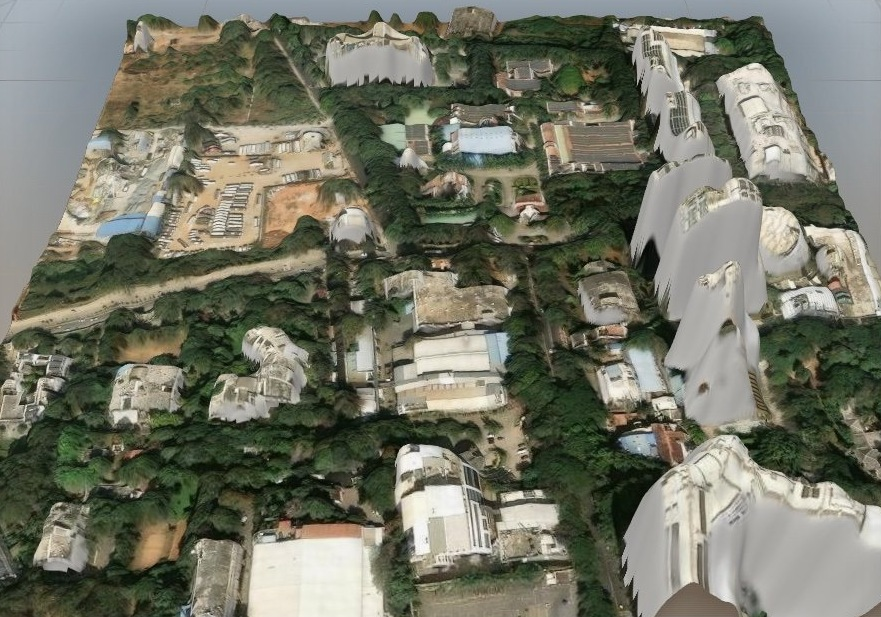
\includegraphics[width=\linewidth]{f1_photo.jpg}\caption{3D model draped with the photograph}\end{subfigure}\hfill
\begin{subfigure}{0.49\linewidth}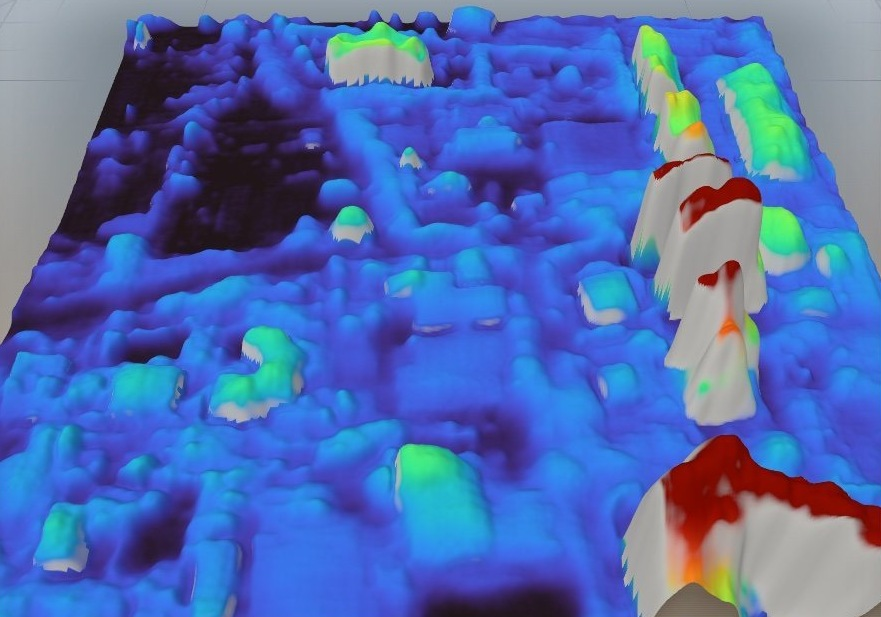
\includegraphics[width=\linewidth]{f1_height.jpg}\caption{Coloured by height above ground}\end{subfigure}
\caption{Bengaluru Electronic City in 3D, built by DepthWizard from one satellite photograph. In (b), colour runs from 0\m{} (dark blue) to 48\m{} (red) above the ground. Heights are drawn at twice their true scale. Imagery: Esri World Imagery, for demonstration only.}
\label{fig:canoas}
\end{figure}

\textbf{Contributions.} In order of importance:
\begin{enumerate}
\item \textbf{A Mamba-based height model (Section~\ref{sec:mamba}).} We built a height model on Mamba~\cite{gu2023mamba}, using NVIDIA's MambaVision~\cite{hatamizadeh2025mambavision} as the image encoder and the two output heads of RS3DAda~\cite{song2024synrs3d}, one for height and one for land cover. Mamba reads an image in one sweep, so its cost grows in step with image area rather than with its square. We train it to reproduce RS3DAda by knowledge distillation~\cite{hinton2015distilling}, with an optional term that learns from true heights, and it is a drop-in replacement in the rest of the system. On 750 test tiles it is 5.2 times faster and nine times smaller than RS3DAda, but not yet as accurate (Section~\ref{sec:compare}).
\item \textbf{Heights tied to sea level and checked by satellite lasers (Section~\ref{sec:terrain}).} We remove rooftops and trees from the free terrain map using the model's own output, level it to NASA ICESat-2 laser points, and add two safety rules learned from real failures.
\item \textbf{Honest error ranges (Section~\ref{sec:conformal}).} Every building receives a range, for example $12\m \pm 6\m$, whose reliability we measured on cities the method never saw.
\item \textbf{Tools for disaster teams (Section~\ref{sec:app}) and a real Indian test (Section~\ref{sec:teesta}).} Eighteen tools, all found from one search box, turn heights into flood, evacuation, landslide and damage maps; we apply the system to the 2023 Teesta flood.
\end{enumerate}

Section~\ref{sec:related} reviews related work, Section~\ref{sec:objectives} states the objectives, Section~\ref{sec:method} describes the method, Section~\ref{sec:app} the application, Section~\ref{sec:data} the test data, Section~\ref{sec:results} the results, and Section~\ref{sec:discussion} discusses limitations and next steps. Table~\ref{tab:terms} explains the technical terms used throughout.

\begin{table}[!htbp]
\centering\small
\caption{Terms used in this paper, in plain words.}
\label{tab:terms}
\begin{tabularx}{\linewidth}{@{}p{3.6cm}Y@{}}
\toprule
Term & Meaning \\
\midrule
Height map (DSM) & A map giving the height of every point, including roofs and tree tops, in metres. \\
Terrain map (DTM) & The height of the bare ground, with buildings and trees removed. \\
Height above ground & How tall an object stands above the ground beneath it. \\
Lidar & Laser scanning from an aircraft or satellite; the most accurate height reference. \\
ICESat-2, GEDI & NASA satellites that measure heights with lasers along narrow tracks. \\
Transformer & A neural network that compares every part of an image with every other part. \\
Mamba & A newer neural network that reads an image in one sweep while keeping a running memory. \\
Distillation & Training a ``student'' model to reproduce the answers of a trained ``teacher'' model. \\
Zero-shot & Tested on places the model never saw in training, with no adjustment. \\
Error (MAE) & The average size of the mistake, in metres; lower is better. \\
Baseline & A simple guess, such as ``everything is flat ground'', that a useful method must beat. \\
CSI & Agreement between a predicted and a real flood map, from 0 (none) to 1 (perfect). \\
\bottomrule
\end{tabularx}
\end{table}

% =====================================================================
\psection{Our Novelty: a Mamba-Based Height Model}{why, how, status}
\label{sec:mamba}

\subsection{Why Mamba}
The published model we start from, RS3DAda~\cite{song2024synrs3d}, reads images with a Transformer, DINOv2 ViT-L~\cite{oquab2023dinov2}. A Transformer cuts the image into small patches and compares every patch with every other patch. This works well, but the work grows with the \emph{square} of the number of patches: doubling the width and height of an area multiplies the comparisons by about sixteen. Satellite scenes are large, so the model must cut them into many small tiles and cannot see far beyond each tile.

Mamba~\cite{gu2023mamba} reads patches one after another while carrying a compact running memory of what it has seen, and chooses at each step what to keep and what to forget; its work grows only in step with the image size. MambaVision~\cite{hatamizadeh2025mambavision} adapts this idea to images: its early stages are convolutions that pick up edges and textures, and its later stages combine Mamba layers with a few Transformer layers, so it still relates distant parts of an image, such as a building and its shadow. Table~\ref{tab:models} sets the two models side by side.

\begin{table}[htbp]
\centering\small
\caption{The published RS3DAda model and our Mamba-based model.}
\label{tab:models}
\begin{tabularx}{\linewidth}{@{}p{3.1cm}YY@{}}
\toprule
 & RS3DAda (published)~\cite{song2024synrs3d} & DepthWizard-Mamba (ours) \\
\midrule
Image encoder & DINOv2 ViT-L/14 Transformer~\cite{oquab2023dinov2} & MambaVision-T, Mamba and attention~\cite{hatamizadeh2025mambavision} \\
How it reads & Every patch against every patch & One sweep with a running memory \\
Cost as area grows & Grows with the square & Grows in step (Mamba layers) \\
Size & 366.5\,M parameters & 40.7\,M parameters \\
Speed (one GPU) & 105 tiles per minute & 546 tiles per minute \\
Graphics memory & 705\,MiB & 78\,MiB \\
Outputs & Height and 8 land-cover classes & The same two heads \\
Tile size & 518 pixels & 512 pixels \\
Training & Synthetic cities + adaptation & Distillation (Eq.~\ref{eq:distill}) or the full recipe \\
Hardware & Any computer, including laptops & NVIDIA graphics card \\
\bottomrule
\end{tabularx}
\end{table}

\subsection{Architecture}
MambaVision produces image features at four scales: $1/4$, $1/8$, $1/16$ and $1/32$ of the input size. Because these already form a pyramid, each scale is passed through a single $1\times1$ projection straight into RS3DAda's dense-prediction heads (DPT~\cite{ranftl2021dpt}), which fuse the scales and return a full-resolution height map and land-cover map (Figure~\ref{fig:arch}). The new model therefore gives exactly the same outputs as the old one, and every later step of DepthWizard runs unchanged.

\begin{figure}[htbp]
\centering
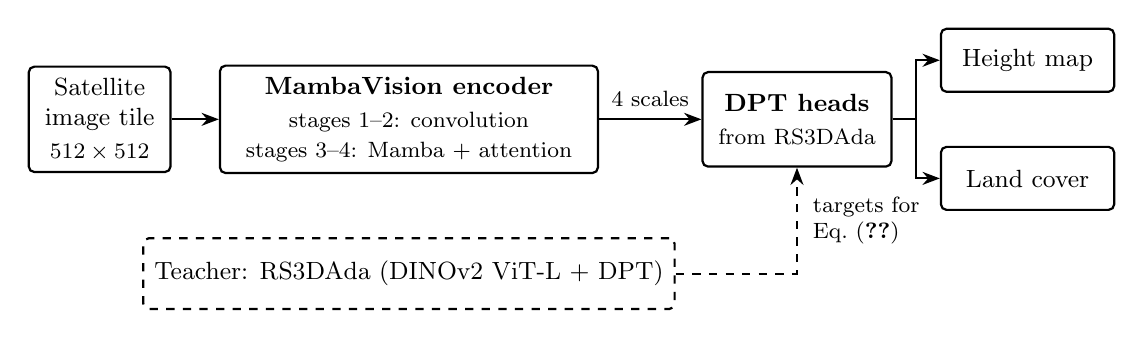
\begin{tikzpicture}[font=\small, node distance=4mm and 6mm,
  blk/.style={draw, thick, rounded corners=2pt, align=center, minimum height=12mm, inner sep=4pt},
  arr/.style={-{Stealth[length=2.2mm]}, thick}]
\node[blk, minimum width=18mm] (img) {Satellite\\image tile\\[1pt]\footnotesize $512\times512$};
\node[blk, right=of img, minimum width=48mm] (enc) {\textbf{MambaVision encoder}\\[1pt]\footnotesize stages 1--2: convolution\\\footnotesize stages 3--4: Mamba + attention};
\node[blk, right=13mm of enc, minimum width=24mm] (dpt) {\textbf{DPT heads}\\[1pt]\footnotesize from RS3DAda};
\node[blk, right=of dpt, yshift=7.5mm, minimum height=8mm, minimum width=22mm] (h) {Height map};
\node[blk, right=of dpt, yshift=-7.5mm, minimum height=8mm, minimum width=22mm] (lc) {Land cover};
\draw[arr] (img) -- (enc);
\draw[arr] (enc) -- node[above=1pt, font=\footnotesize]{4 scales} (dpt);
\draw[arr] (dpt.east) -- ++(3mm,0) |- (h.west);
\draw[arr] (dpt.east) -- ++(3mm,0) |- (lc.west);
\node[blk, dashed, below=8mm of enc, minimum width=48mm, minimum height=9mm] (t) {Teacher: RS3DAda (DINOv2 ViT-L + DPT)};
\draw[arr, dashed] (t.east) -| node[pos=0.75, right=2pt, font=\footnotesize, align=left]{targets for\\Eq.~(\ref{eq:distill})} (dpt.south);
\end{tikzpicture}
\caption{The Mamba-based height model. The encoder's four feature scales go directly into the same two output heads that RS3DAda uses; during training, RS3DAda's own answers serve as targets.}
\label{fig:arch}
\end{figure}

\subsection{Training by distillation}
Training a height model from scratch needs very large labelled datasets. Instead, the Mamba model (the student, S) looks at unlabelled satellite images and learns to give the same answers as RS3DAda (the teacher, T)~\cite{hinton2015distilling}. With predicted heights $\hat h$, land-cover scores $z$ and the softmax $\sigma$, its training objective is
\begin{equation}
\mathcal{L} \;=\; \ell_{1}^{\mathrm{s}}\!\bigl(\hat h_{\mathrm S},\hat h_{\mathrm T}\bigr)
\;+\; \lambda\,\tau^{2}\,\mathrm{KL}\!\bigl(\sigma(z_{\mathrm T}/\tau)\,\big\|\,\sigma(z_{\mathrm S}/\tau)\bigr)
\;+\; \gamma\,\ell_{1}^{\mathrm{s}}\!\bigl(\hat h_{\mathrm S},h_{\mathrm{label}}\bigr),
\label{eq:distill}
\end{equation}
where $\ell_1^{\mathrm s}$ is the smooth-L1 loss. In words: the first term penalises differences in height from the teacher; the second makes the student's land-cover answers match the teacher's, softened by a temperature $\tau$ so that the student also learns how sure the teacher was; and the optional third term uses true heights from the synthetic SynRS3D cities, which lets the student improve on the teacher instead of copying its faults. Table~\ref{tab:train} lists the settings. The same model can also be trained with RS3DAda's full recipe of synthetic data plus adaptation to real images.

\begin{table}[!htbp]
\centering\small
\caption{Training settings for the Mamba model.}
\label{tab:train}
\begin{tabularx}{0.82\linewidth}{@{}p{4.4cm}Y@{}}
\toprule
Setting & Value \\
\midrule
Teacher & RS3DAda, released weights \\
Training images & SynRS3D tiles; 2\% held out for validation \\
Crops and augmentation & 512\,px random crops, flips and $90^\circ$ turns \\
Steps, batch size & 20{,}000 steps, 8 images per step \\
Optimiser & AdamW, weight decay $10^{-4}$ \\
Learning rate & heads $10^{-4}$, encoder $10^{-5}$; 500-step warm-up, then cosine \\
Loss weights (Eq.~\ref{eq:distill}) & $\lambda=0.5$, $\tau=2$; $\gamma=0$, or $\gamma>0$ with labels \\
Validation & height error against the teacher every 1{,}000 steps \\
\bottomrule
\end{tabularx}
\end{table}

\subsection{First results}
The first Mamba student was trained with the settings of Table~\ref{tab:train} and tested on the same 750 tiles as RS3DAda (Section~\ref{sec:compare}). It delivers the efficiency we designed it for: it has nine times fewer parameters, needs nine times less graphics memory and processes 546 tiles per minute against RS3DAda's 105 on the same graphics card (Table~\ref{tab:models}). It is not yet as accurate. Its average error is 7.20\m{} on the aerial lidar tiles against 3.90\m{} for RS3DAda, worse than the flat-ground guess there (5.65\m), and 8.70\m{} and 3.39\m{} on the Atlanta and Buenos Aires satellite tiles against 5.91\m{} and 1.86\m{} for RS3DAda. Most of the gap is in finding \emph{where} objects are: even after each tile's scale and offset are corrected, its correlation with the true heights is 0.29 against 0.61. The deployed app therefore keeps RS3DAda, and closing this gap with longer training and the true-height term of Eq.~(\ref{eq:distill}) is our first next step.

% =====================================================================
\psection{Related Work}{what already exists}
\label{sec:related}

\textbf{Height from one image.} Transformers with dense-prediction heads~\cite{ranftl2021dpt} estimate depth from a single photograph. RS3DAda~\cite{song2024synrs3d} adapted this to satellite images by training on SynRS3D, a large set of computer-generated cities, then adjusting to real images without labels. General-purpose depth models such as Depth Anything~V2~\cite{yang2024dav2} are trained on ordinary photographs; we compare against them in Section~\ref{sec:compare}. Mamba~\cite{gu2023mamba} and MambaVision~\cite{hatamizadeh2025mambavision} are recent alternatives to Transformers; to our knowledge, no ready-to-use satellite height model built on them has been released.

\textbf{Terrain and lasers.} Copernicus GLO-30~\cite{esa2021glo30} is a free worldwide terrain map at 30\m; FABDEM~\cite{hawker2022fabdem} removes buildings and forest from it for non-commercial use. NASA's ICESat-2~\cite{neumann2019icesat2,neuenschwander2019atl08} and GEDI~\cite{dubayah2020gedi} measure ground and tree-top heights with lasers along narrow tracks, and Meta's canopy map~\cite{tolan2024canopy} gives tree heights worldwide at 1\m. Song \emph{et al.}~\cite{song2025sparse} recently showed that sparse ICESat-2 points can correct single-image height maps, which supports the levelling step we use for terrain.

\textbf{Disaster modelling.} A simplified shallow-water model~\cite{bates2010inertial} predicts how floods spread; radar images split into water and land by Otsu's method~\cite{otsu1979} show where floods really were; and the Indian Standard IS~14496~\cite{bis14496} classifies slopes by landslide risk. Table~\ref{tab:approaches} compares the main ways of obtaining heights.

\begin{table}[!htbp]
\centering\small
\caption{Ways of obtaining heights for disaster response.}
\label{tab:approaches}
\begin{tabularx}{\linewidth}{@{}YYccc@{}}
\toprule
Approach & Needs & Detail & Sea level & Error stated \\
\midrule
Aircraft lidar survey & A survey flight & Very fine & Yes & Yes \\
Stereo satellite pair & Two matched images & Fine & Yes & Partly \\
GLO-30, FABDEM~\cite{esa2021glo30,hawker2022fabdem} & Nothing (free) & 30\m & Yes & No \\
RS3DAda~\cite{song2024synrs3d} & One image & Pixel & No & No \\
\textbf{DepthWizard (ours)} & One image + free data & Pixel & Yes & Yes, measured \\
\bottomrule
\end{tabularx}
\end{table}

% =====================================================================
\psection{Objectives}{what success means}
\label{sec:objectives}

Each objective in Table~\ref{tab:objectives} had its test fixed before the work began.

\begin{table}[!htbp]
\centering\small
\caption{Objectives and how each is measured.}
\label{tab:objectives}
\begin{tabularx}{\linewidth}{@{}lYY@{}}
\toprule
\# & Objective & How success is measured \\
\midrule
O1 & A height for every pixel of one image & Smaller error than a flat-ground guess on unseen data \\
O2 & Heights in metres above sea level & Closer to laser-measured ground than the free terrain map \\
O3 & Correction from a few surveyed points & Error reported each time, checked on a left-out point \\
O4 & Checking inside the app & Error figures per scene and per type of land \\
O5 & An honest error range on each building & Range holds 90\% of the time on unseen cities \\
O6 & Disaster tools that are easy to find & Every tool opens from one search box \\
O7 & Works offline on an ordinary laptop & Measured time for one full scene \\
O8 & A more efficient height model (Mamba) & Faster and smaller than RS3DAda on the same tests; accuracy compared \\
\bottomrule
\end{tabularx}
\end{table}

% =====================================================================
\psection{Method}{from photograph to checked 3D map}
\label{sec:method}

\subsection{Pipeline}
A scene goes through seven steps (Figure~\ref{fig:pipeline}). An ordinary PNG or JPEG photograph gives heights above the ground; a GeoTIFF, which carries its location, continues to heights above sea level.

\begin{figure}[!htbp]
\centering
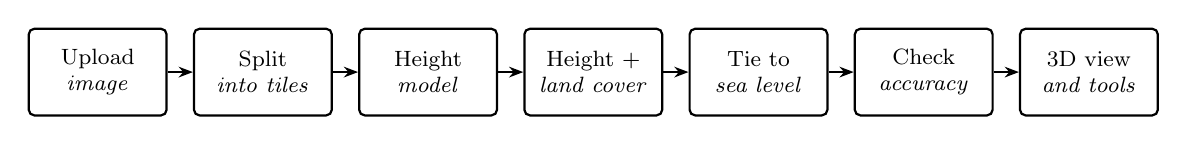
\begin{tikzpicture}[font=\footnotesize, node distance=3.2mm,
  st/.style={draw, thick, rounded corners=2pt, align=center, minimum width=17.5mm, minimum height=11mm, inner sep=2pt},
  arr/.style={-{Stealth[length=1.8mm]}, thick}]
\node[st] (a) {Upload\\\textit{image}};
\node[st, right=of a] (b) {Split\\\textit{into tiles}};
\node[st, right=of b] (c) {Height\\\textit{model}};
\node[st, right=of c] (d) {Height +\\\textit{land cover}};
\node[st, right=of d] (e) {Tie to\\\textit{sea level}};
\node[st, right=of e] (f) {Check\\\textit{accuracy}};
\node[st, right=of f] (g) {3D view\\\textit{and tools}};
\foreach \x/\y in {a/b,b/c,c/d,d/e,e/f,f/g} \draw[arr] (\x) -- (\y);
\end{tikzpicture}
\caption{From one photograph to a checked 3D map. Tiles overlap by half, and each is read four times (original and flipped) to smooth the result.}
\label{fig:pipeline}
\end{figure}

\subsection{From height above ground to height above sea level}
\label{sec:terrain}
The model gives the height $h$ of each point $x$ above the ground beneath it. Adding the height of the ground itself gives the height above sea level:
\begin{equation}
\mathrm{DSM}(x) \;=\; \mathrm{DTM}(x) \;+\; h(x).
\label{eq:dsm}
\end{equation}
The ground map starts as GLO-30~\cite{esa2021glo30}, which in towns sits on rooftops. In each 30\m{} square we therefore subtract the average building and tree height the model found, and where a square is mostly roofs or trees we fill it from its neighbours. We then shift the whole map up or down to match ICESat-2 laser points that reached the ground~\cite{neuenschwander2019atl08}. Two safety rules came from observed failures: we refuse to shift when only one laser track crosses the scene, and we discard ``ground'' laser points that sit on a roof. If the user has surveyed $K$ points of known elevation $z_k$ at positions $(x_k,y_k)$, the map value $\hat z_k$ there is corrected with the best-fitting level, scale and tilt:
\begin{equation}
\min_{a,b,c,d}\; \sum_{k=1}^{K} \bigl(z_k - a - b\,\hat z_k - c\,x_k - d\,y_k\bigr)^2 .
\label{eq:gcp}
\end{equation}
One point sets only the level $a$; two or three also set the scale $b$; four or more also set the tilt $c,d$. A leave-one-out error is reported with every fit.

\subsection{Correcting tree heights}
The model sees trees at only 18--60\% of their true height. Trees can therefore take their height from Meta's canopy map~\cite{tolan2024canopy}, or be scaled up by a factor learned from the GEDI laser shots~\cite{dubayah2020gedi} that fall on trees,
\begin{equation}
s_{\mathrm{tree}} \;=\; \operatorname*{median}_{k}\; \frac{H_k^{\mathrm{GEDI}}}{\hat h_k},
\label{eq:tree}
\end{equation}
that is, the typical ratio between the laser's tree height $H_k$ and the model's $\hat h_k$ at the same spots.

\subsection{An error range for every building}
\label{sec:conformal}
Each tile is read four times; how much the four answers disagree, $u$, hints at how unsure the model is. Split conformal prediction~\cite{lei2018conformal} turns this hint into a range that holds a stated share of the time. On $n$ buildings with known heights we compute the errors $e_i$ and set
\begin{equation}
r_i = \frac{|e_i|}{u_i+u_0},\qquad
\hat q = r_{(\lceil (n+1)(1-\alpha)\rceil)},\qquad
C(x) = \bigl[\,\hat h(x) \pm \hat q\,\bigl(u(x)+u_0\bigr)\bigr],
\label{eq:conformal}
\end{equation}
where $r_{(k)}$ is the $k$-th smallest score, so that the range $C(x)$ should contain the true height 90\% of the time ($\alpha=0.1$, $u_0=0.25\m$). We then test that promise on cities that were not used to set it.

\subsection{Disaster models}
For a simple flood, every place below a chosen water level that is connected to the river or the scene edge is marked wet. For water that flows over time we use the model of Bates \emph{et al.}~\cite{bates2010inertial}, which moves water between neighbouring cells according to the slope of the water surface $\eta$, the flow depth $h_f$ and the ground roughness $n$:
\begin{equation}
q_{t+\Delta t} \;=\; \frac{q_t - g\,h_f\,\Delta t\,\partial\eta/\partial x}{1 + g\,\Delta t\,n^2\,|q_t|\,/\,h_f^{7/3}},
\label{eq:flow}
\end{equation}
where $q$ is the discharge per unit width and $g$ the gravitational acceleration. We added limits so that no cell gives away more water than it holds. To compare a flood prediction with reality we use a real flood map, from a mask or from a radar image split into water and land~\cite{otsu1979}, and the critical success index
\begin{equation}
\mathrm{CSI} \;=\; \frac{TP}{TP+FP+FN},
\label{eq:csi}
\end{equation}
where $TP$ counts cells both maps call wet, and $FP$ and $FN$ the cells only one of them calls wet. Evacuation routes are the cheapest paths~\cite{dijkstra1959} that avoid steep slopes, deep water and buildings; landslide risk follows IS~14496~\cite{bis14496}. All outputs are labelled as scenarios, not forecasts.

% =====================================================================
\psection{The Application}{pages and tools}
\label{sec:app}

DepthWizard runs on an ordinary laptop. A Python server runs the height model, terrain and laser steps and stores heavy data per scene, so a scene opened once works without internet; the browser interface uses three.js~\cite{threejs} for the 3D view. The site has a home page, a scene library and six working pages that follow the disaster cycle: explore the heights, check them, prepare before a disaster, respond during it, plan relief and assess the damage (Figure~\ref{fig:pages}). Every tool is a panel that switches on in place and can also be found by typing its name in a search box (\textit{Ctrl\,K}). Results export as GeoTIFF, 3D model (GLB), GeoJSON and CityJSON files that open in QGIS, ArcGIS or Bhuvan. Table~\ref{tab:tools} lists the tools, and Figure~\ref{fig:tools} shows several of them running on real scenes.

\begin{figure}[p]
\centering
\begin{subfigure}{0.485\linewidth}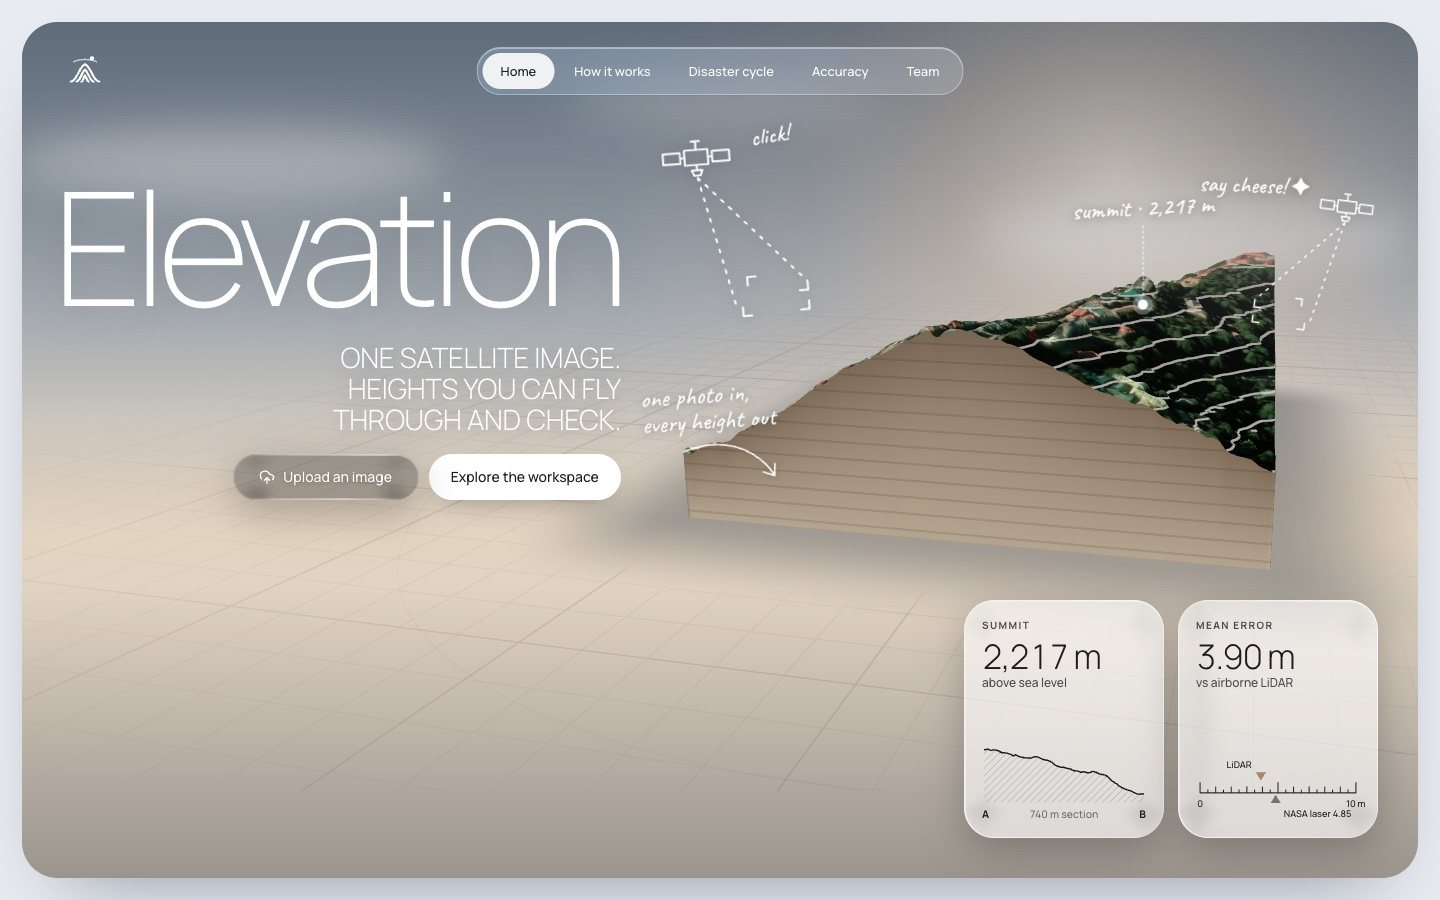
\includegraphics[width=\linewidth]{p_home.jpg}\caption{Home}\end{subfigure}\hfill
\begin{subfigure}{0.485\linewidth}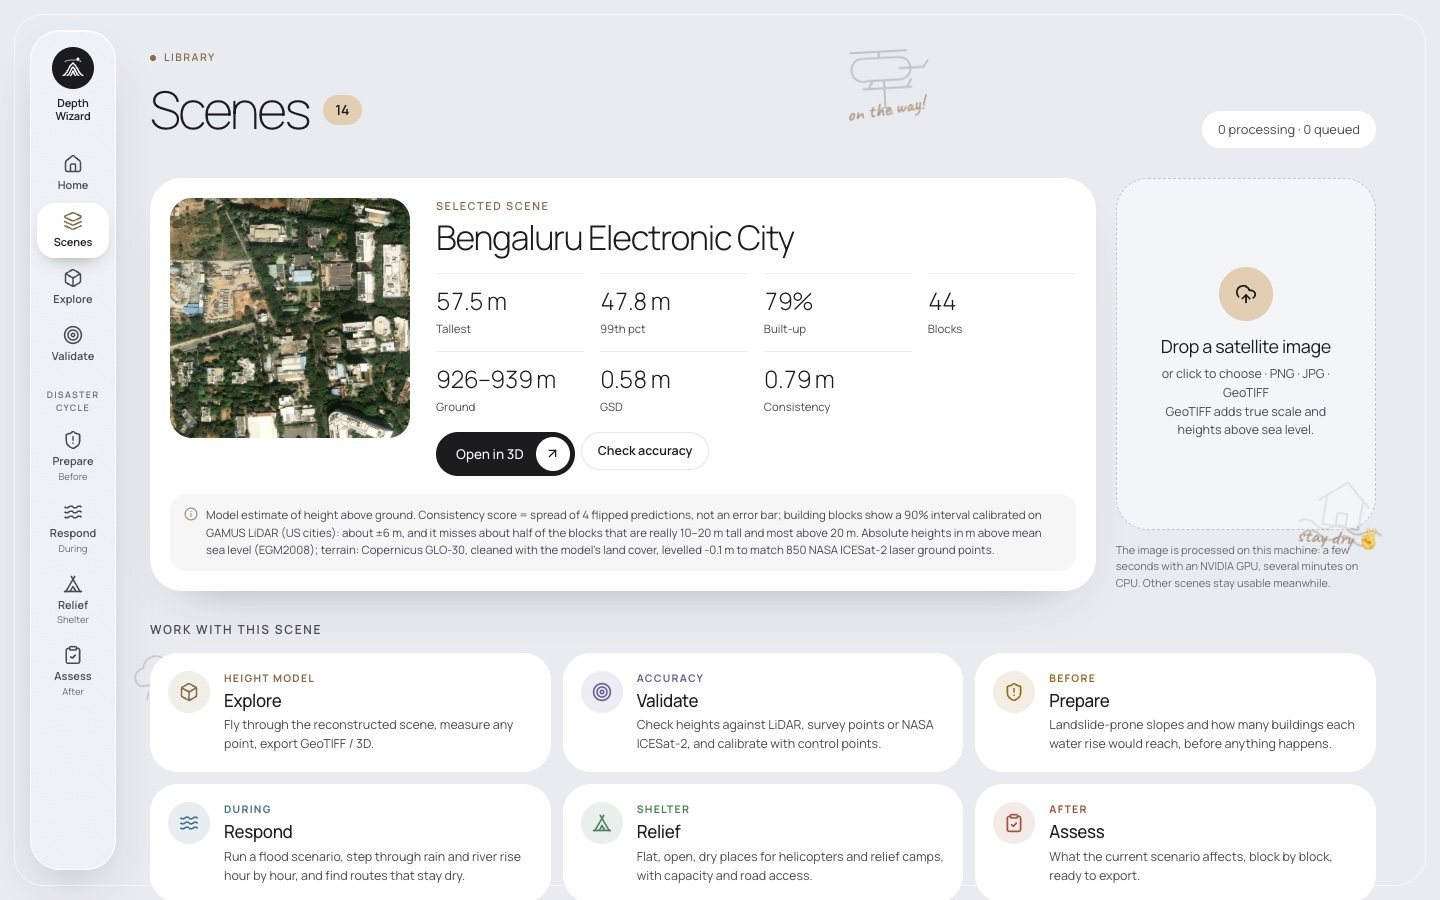
\includegraphics[width=\linewidth]{p_scenes.jpg}\caption{Scenes: library and upload}\end{subfigure}\\[6pt]
\begin{subfigure}{0.485\linewidth}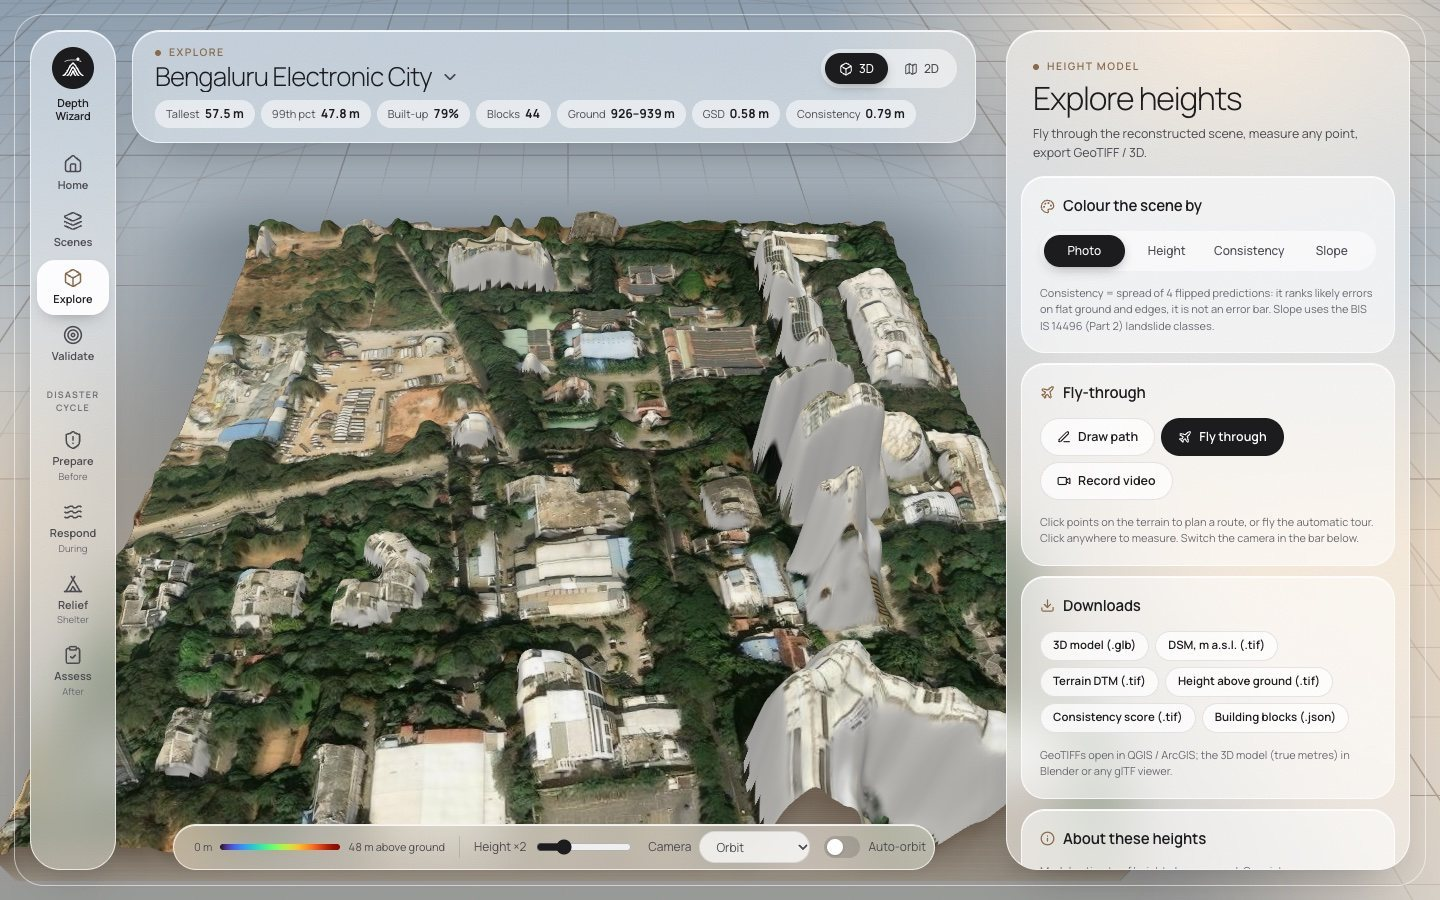
\includegraphics[width=\linewidth]{p_explore.jpg}\caption{Explore: 3D heights and fly-through}\end{subfigure}\hfill
\begin{subfigure}{0.485\linewidth}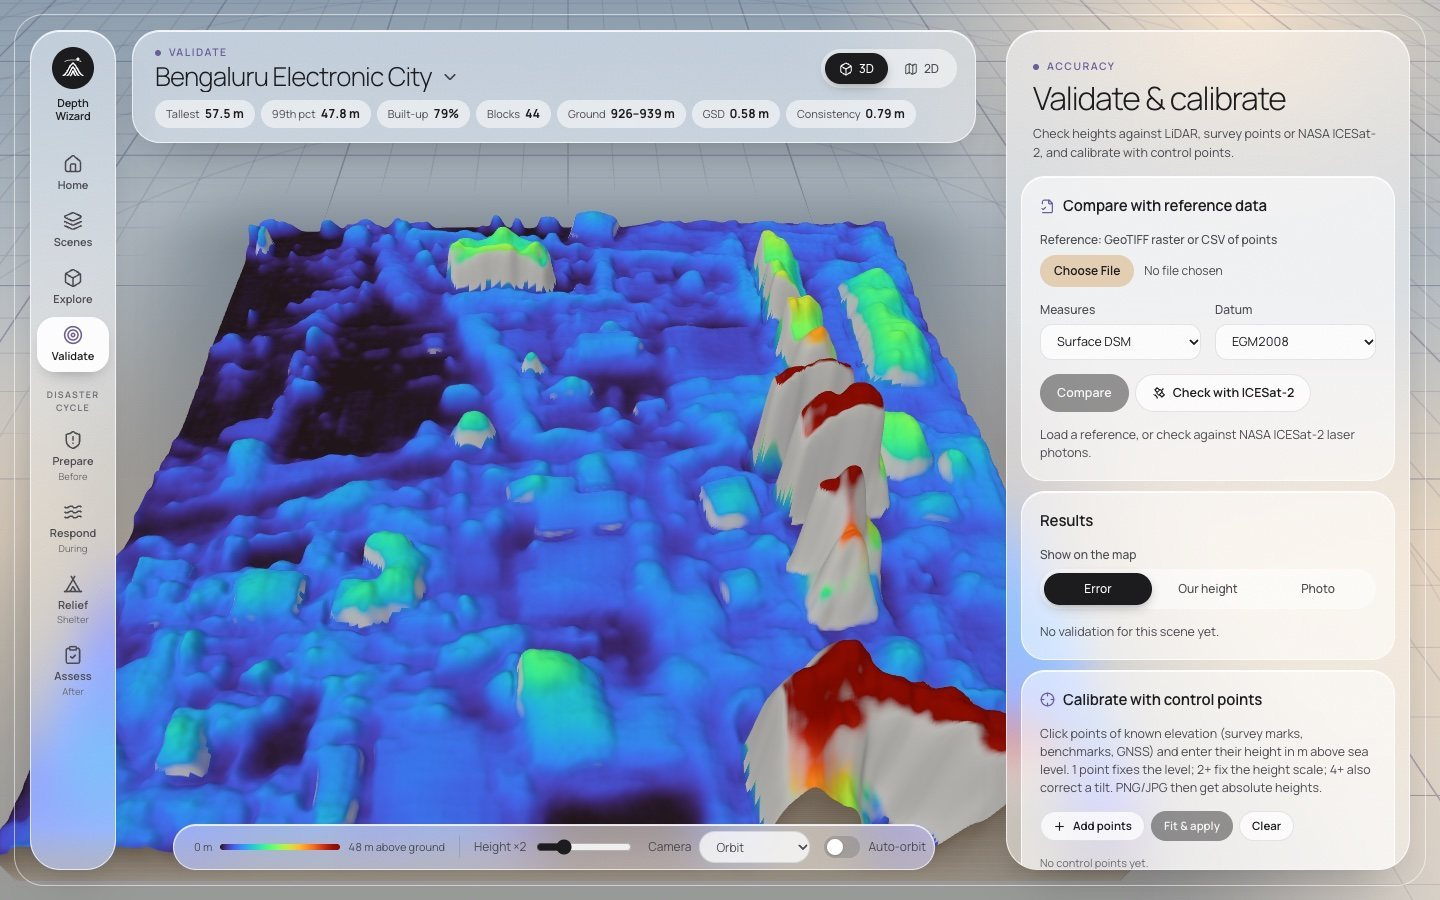
\includegraphics[width=\linewidth]{p_validate.jpg}\caption{Validate: check against references}\end{subfigure}\\[6pt]
\begin{subfigure}{0.485\linewidth}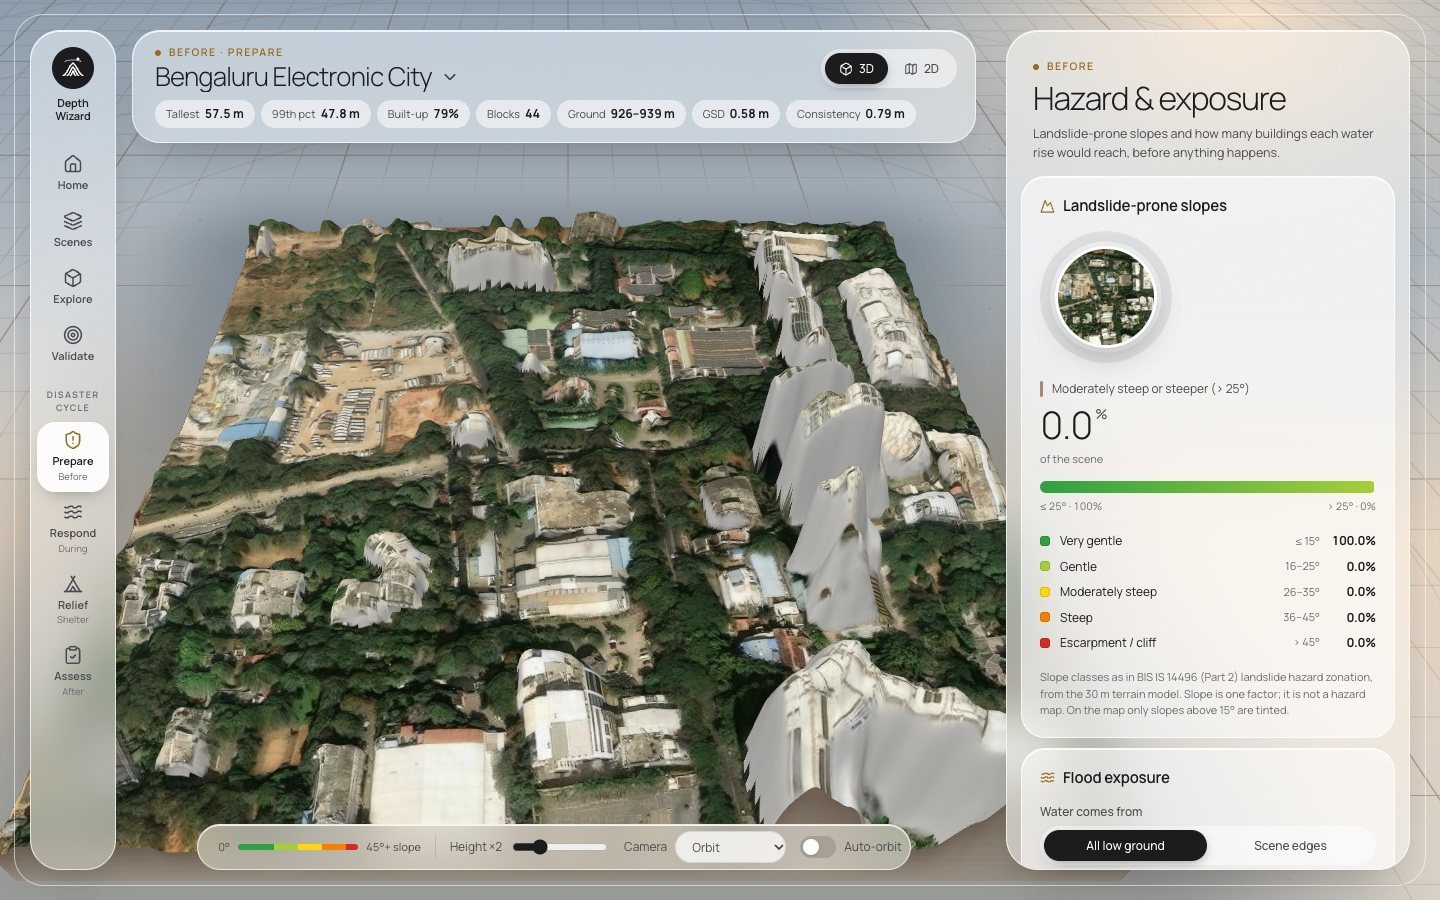
\includegraphics[width=\linewidth]{p_prepare.jpg}\caption{Prepare: risky slopes and water rise}\end{subfigure}\hfill
\begin{subfigure}{0.485\linewidth}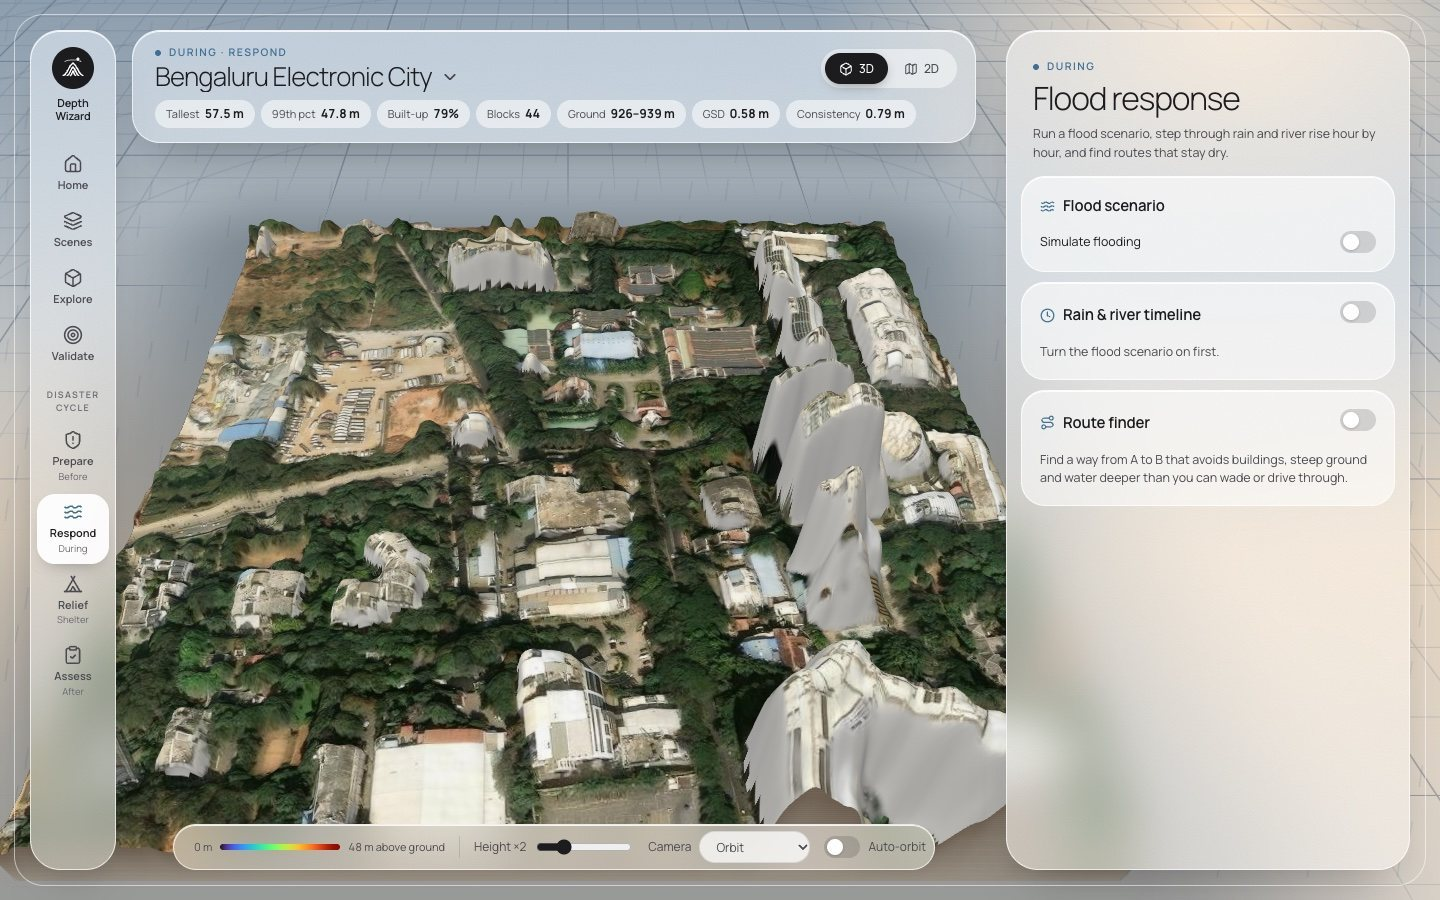
\includegraphics[width=\linewidth]{p_respond.jpg}\caption{Respond: flood scenario and routes}\end{subfigure}\\[6pt]
\begin{subfigure}{0.485\linewidth}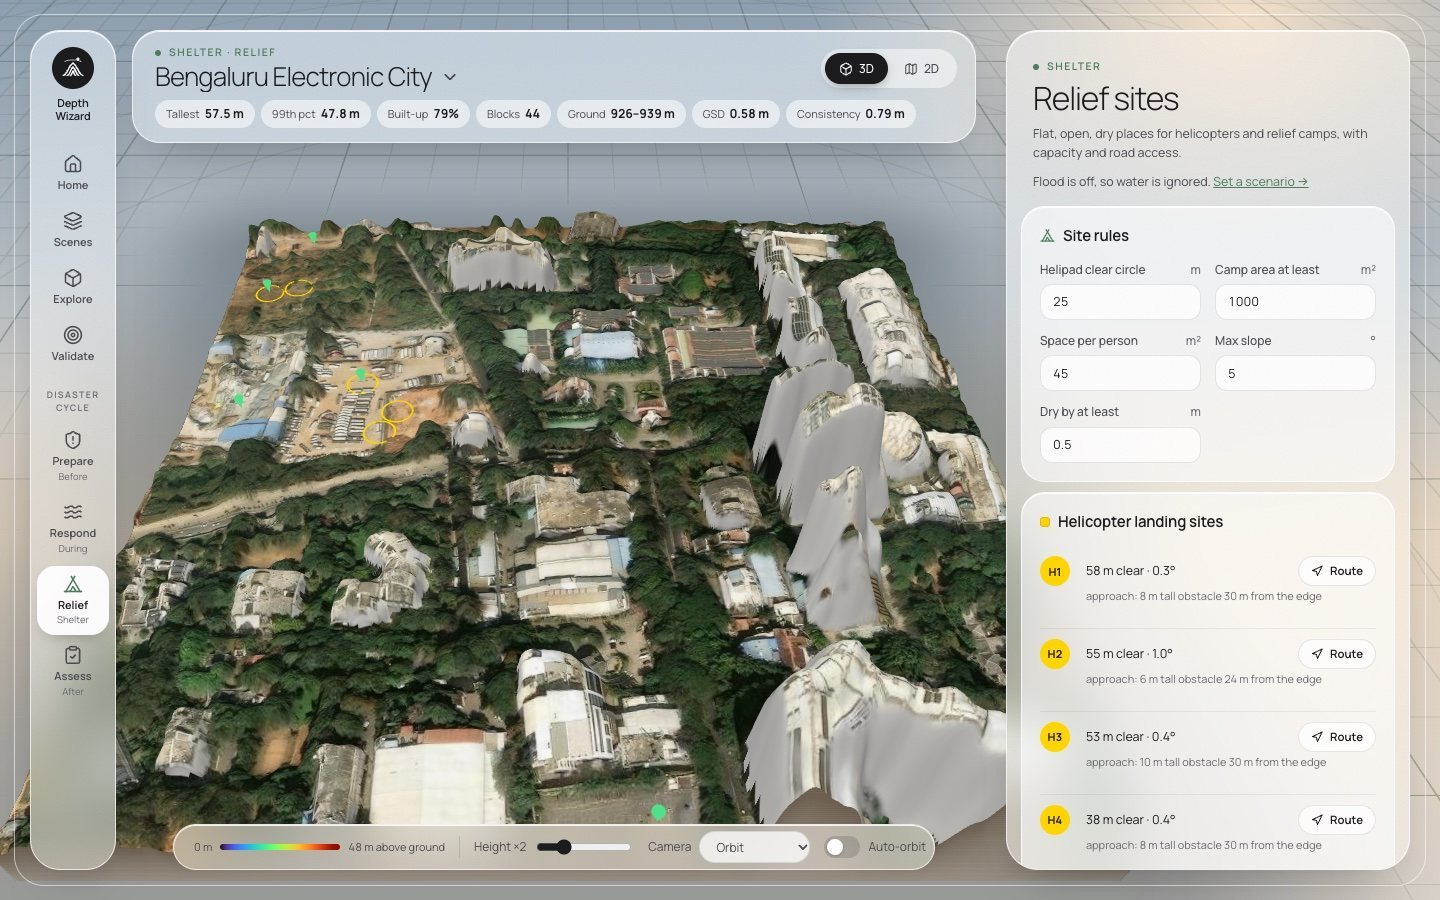
\includegraphics[width=\linewidth]{p_relief.jpg}\caption{Relief: helipad and camp sites}\end{subfigure}\hfill
\begin{subfigure}{0.485\linewidth}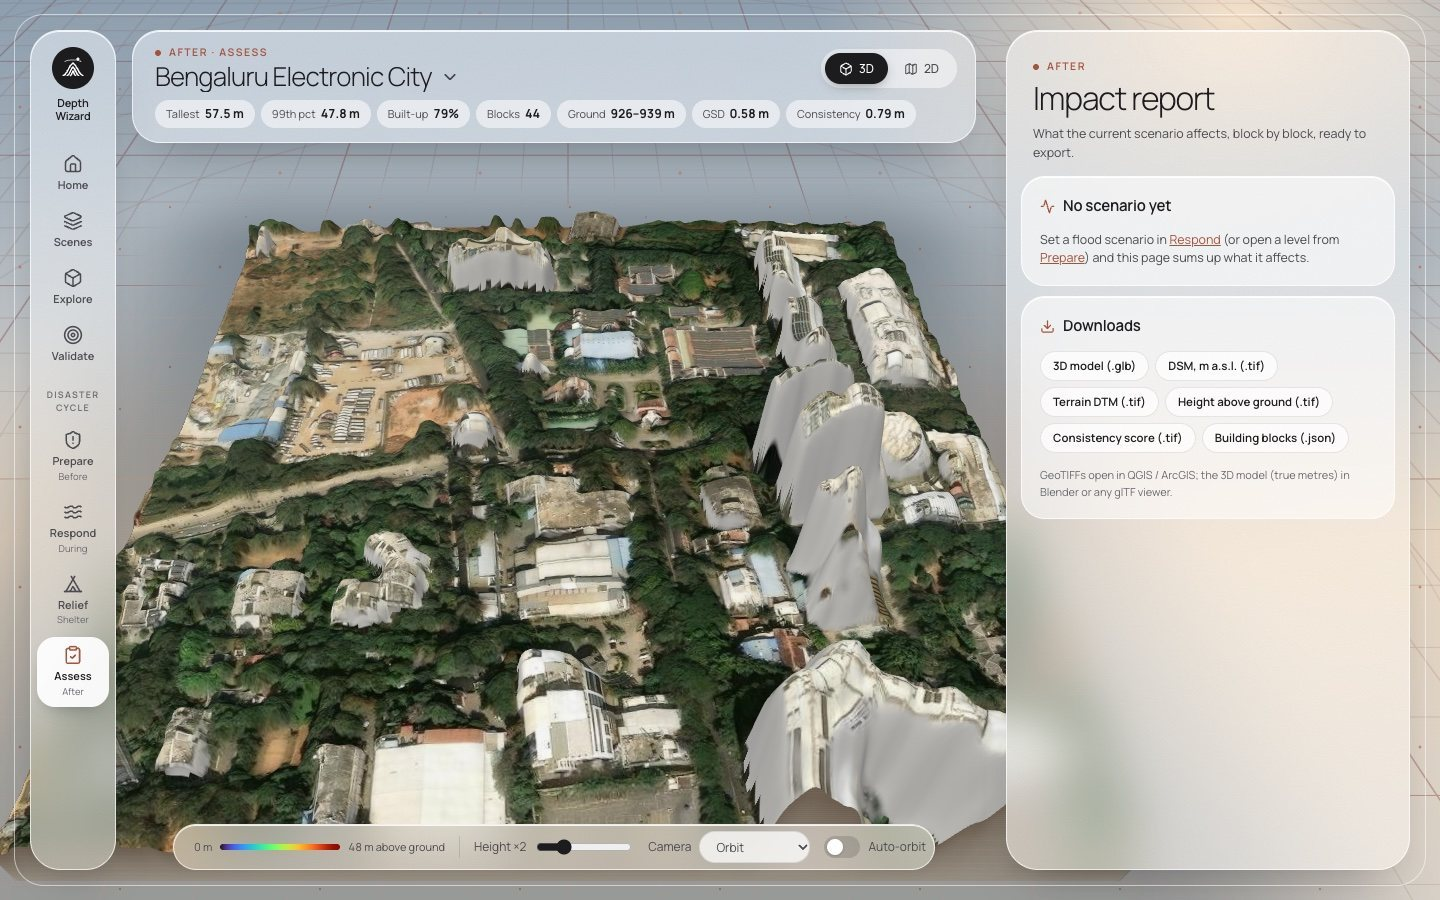
\includegraphics[width=\linewidth]{p_assess.jpg}\caption{Assess: impact report}\end{subfigure}
\caption{The application on a real scene, Bengaluru Electronic City, built from one satellite image.}
\label{fig:pages}
\end{figure}

\begin{table}[!htbp]
\centering\small
\caption{The eighteen tools and the question each answers.}
\label{tab:tools}
\begin{tabularx}{\linewidth}{@{}p{4.2cm}Y@{}}
\toprule
Tool & Question it answers \\
\midrule
\multicolumn{2}{@{}l}{\textit{Explore}} \\
Line of sight & What can be seen from this mast, tower or camera? \\
Volume and area & How much debris is in this pile, or water in this pond? \\
Drone flight plan & Which route keeps a drone safely above every roof? \\
Rooftop solar & How much power could each roof produce, allowing for shade? \\
Map overlay & Where are the streets and names on top of the 3D view? \\
Mosaic & How do neighbouring scenes join into one larger area? \\
\addlinespace
\multicolumn{2}{@{}l}{\textit{Validate and calibrate}} \\
Heights from shadows & Do shadow lengths in the photograph confirm the heights? \\
Tree and tall-object fix & Can the weakest heights be corrected from other sources (Eq.~\ref{eq:tree})? \\
Error bars & How far could each height be off (Eq.~\ref{eq:conformal})? \\
Terrain source & Can I use my own, better ground map? \\
GPS and field points & Can points measured on the ground correct the map (Eq.~\ref{eq:gcp})? \\
\addlinespace
\multicolumn{2}{@{}l}{\textit{Prepare, Respond, Relief, Assess}} \\
Landslide risk & Which slopes may fail in heavy rain? \\
People at risk & How many people live in the affected buildings? \\
Observed flood & How well does the predicted flood match a real flood map (Eq.~\ref{eq:csi})? \\
Flowing water & Where does the water go, hour by hour (Eq.~\ref{eq:flow})? \\
Evacuation plan & Which camp should each family go to, and by which route? \\
Damage before/after & Which buildings collapsed and which are new? \\
Situation report & What does a decision maker need on one page? \\
\bottomrule
\end{tabularx}
\end{table}

\begin{figure}[p]
\centering
\begin{subfigure}{0.485\linewidth}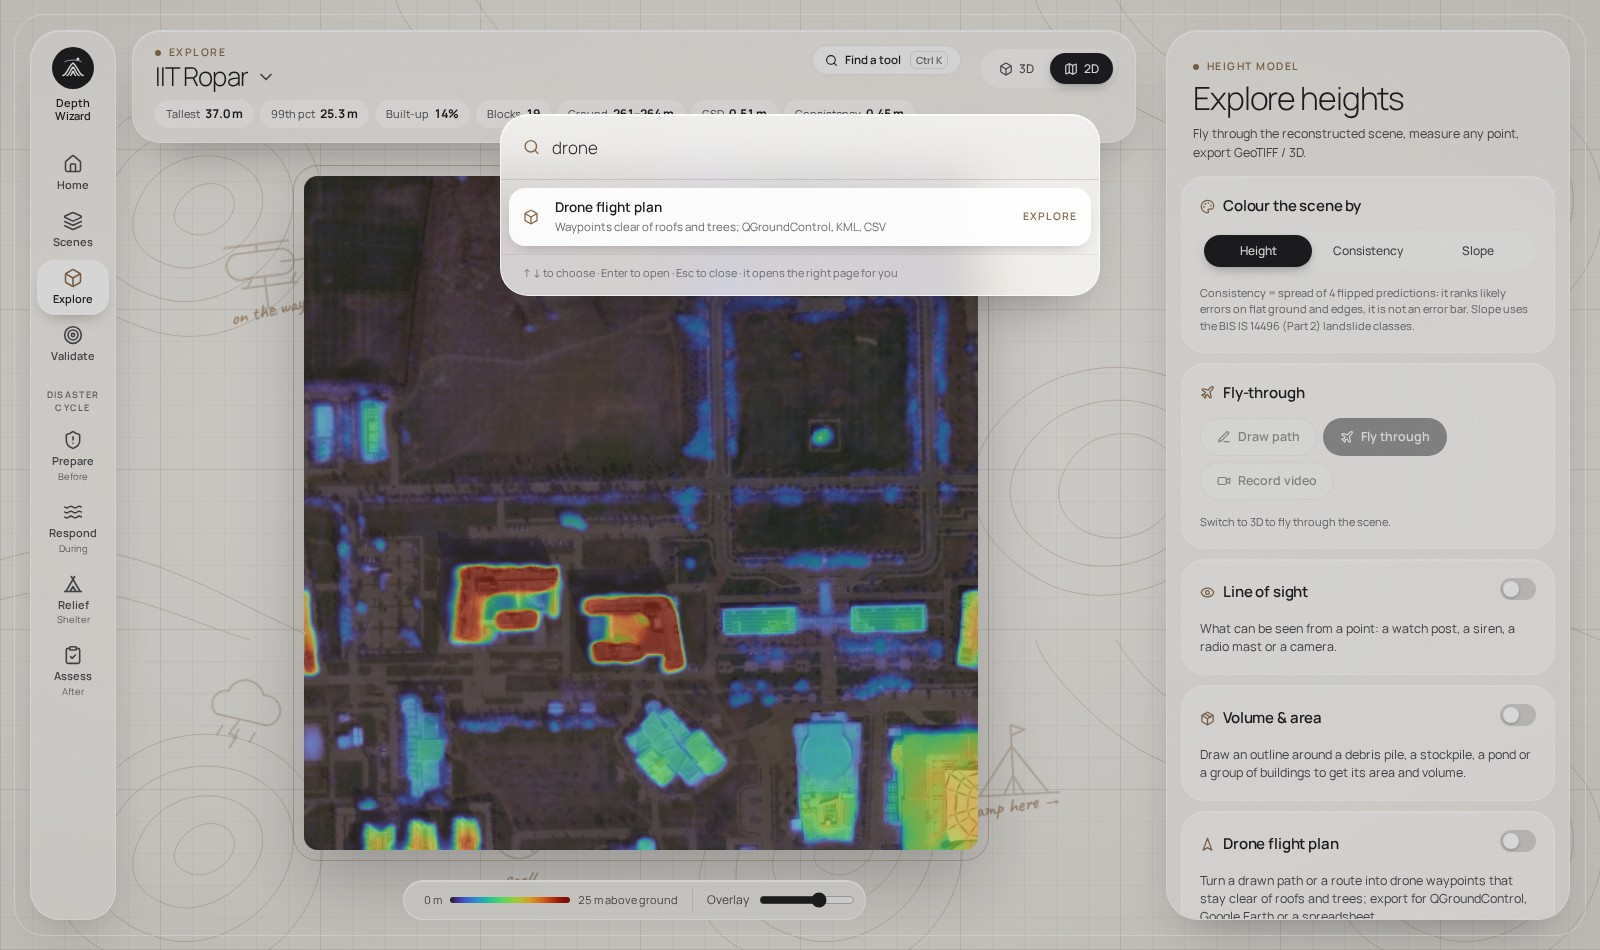
\includegraphics[width=\linewidth]{s_find.jpg}\caption{Tool finder: typing ``drone''}\end{subfigure}\hfill
\begin{subfigure}{0.485\linewidth}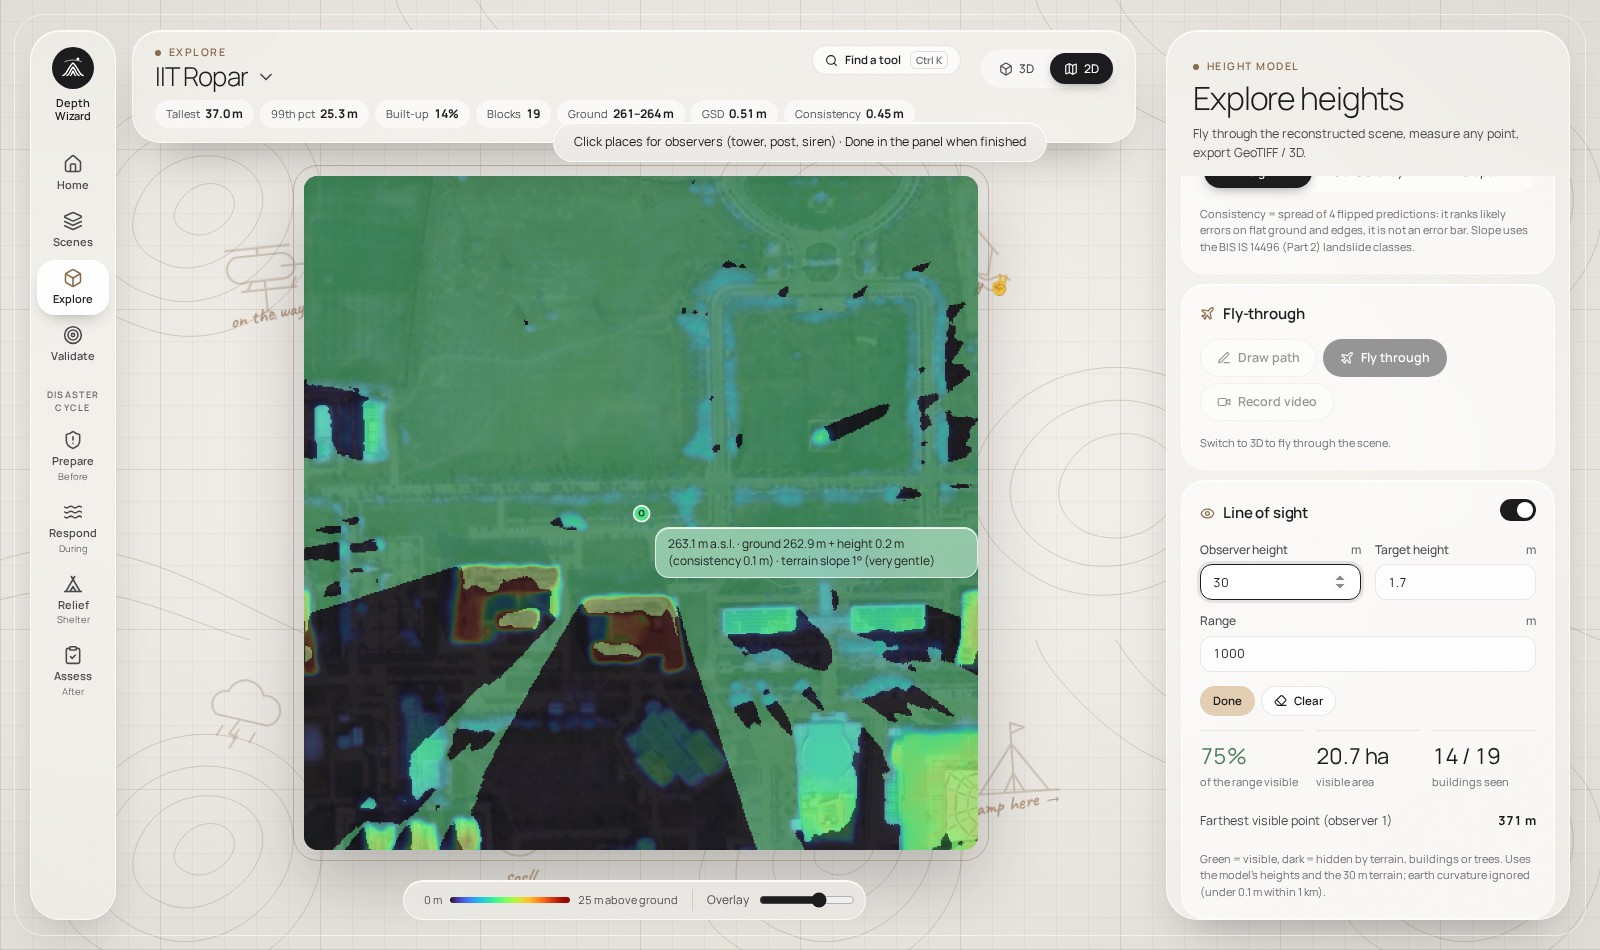
\includegraphics[width=\linewidth]{s_los.jpg}\caption{Line of sight from a 30\m{} mast}\end{subfigure}\\[6pt]
\begin{subfigure}{0.485\linewidth}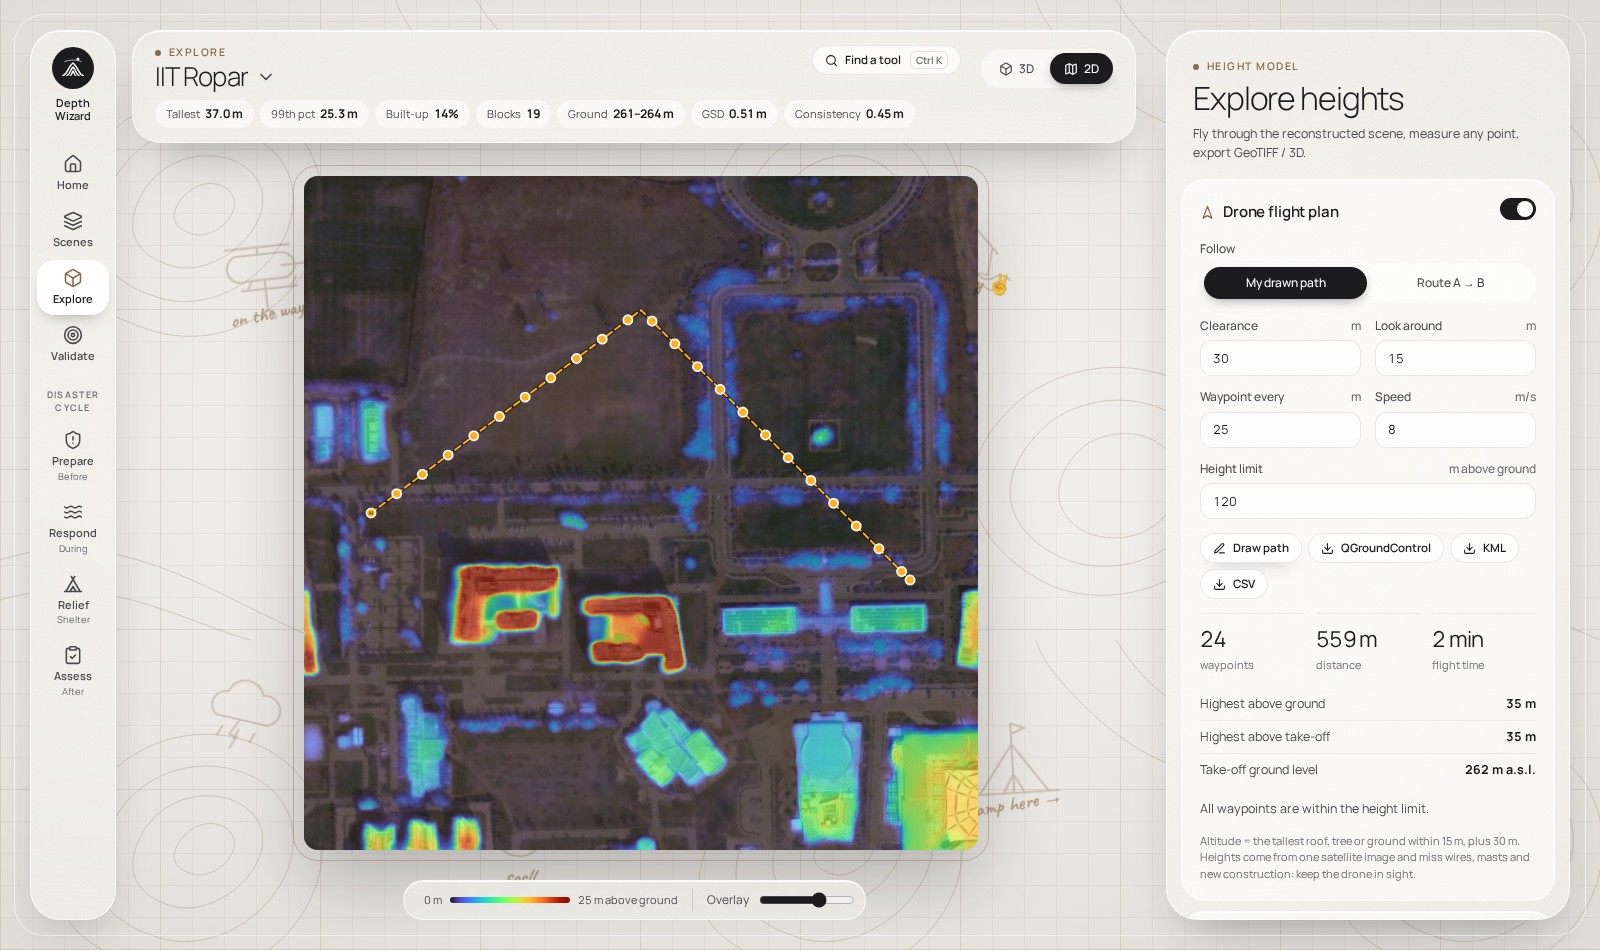
\includegraphics[width=\linewidth]{s_drone.jpg}\caption{Drone flight plan clear of every roof}\end{subfigure}\hfill
\begin{subfigure}{0.485\linewidth}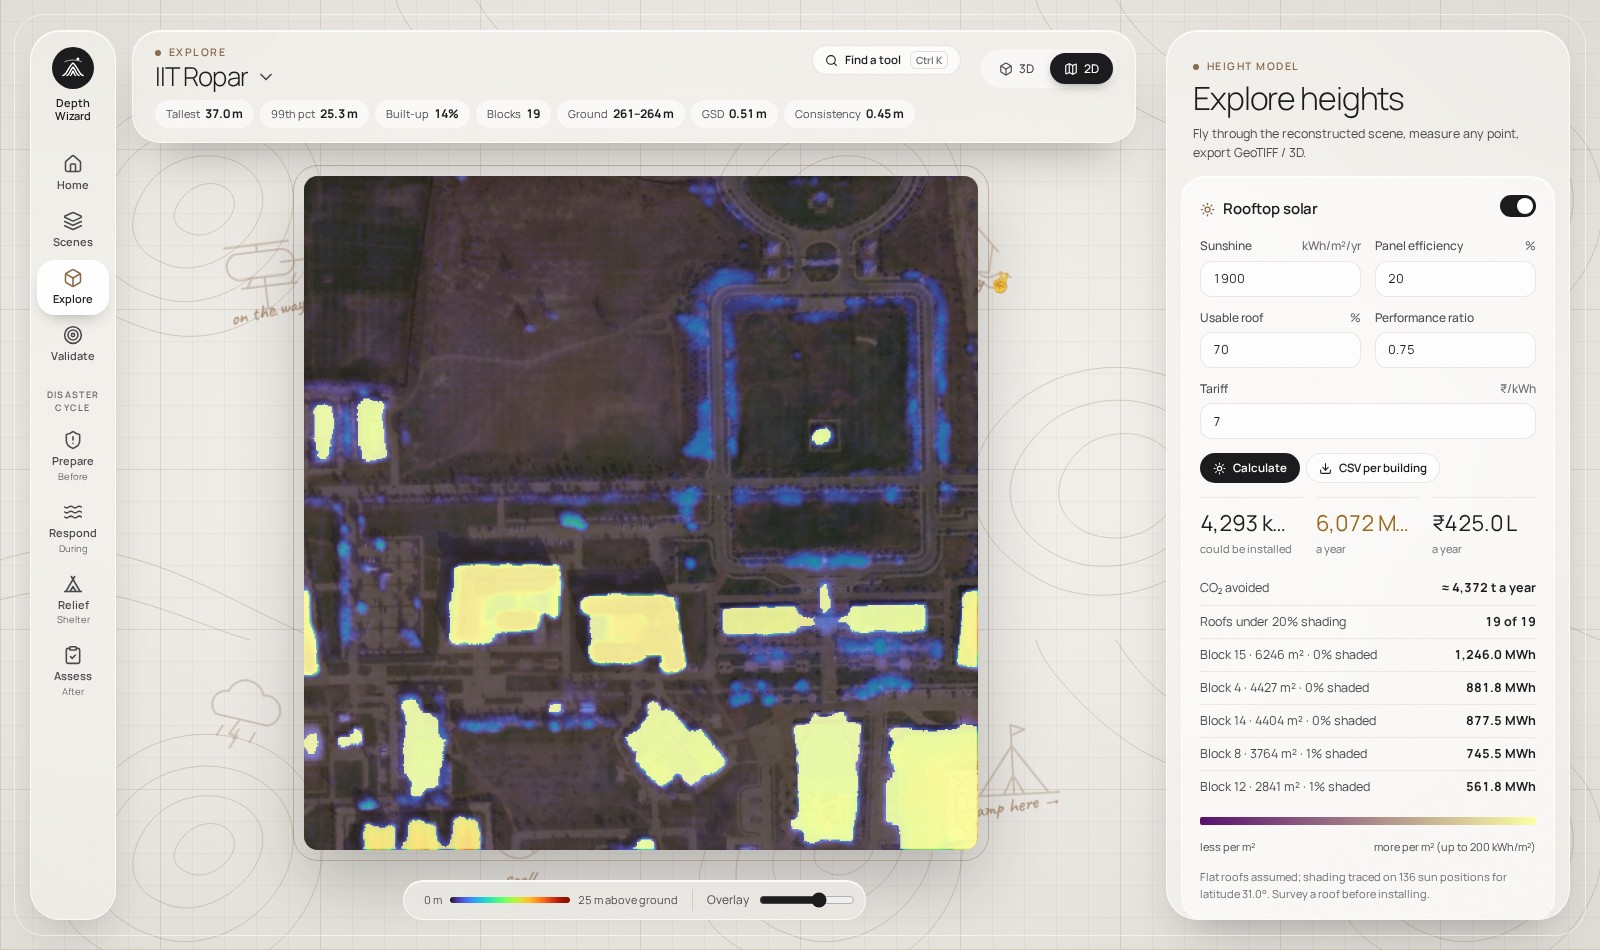
\includegraphics[width=\linewidth]{s_solar.jpg}\caption{Rooftop solar yield with shading}\end{subfigure}\\[6pt]
\begin{subfigure}{0.485\linewidth}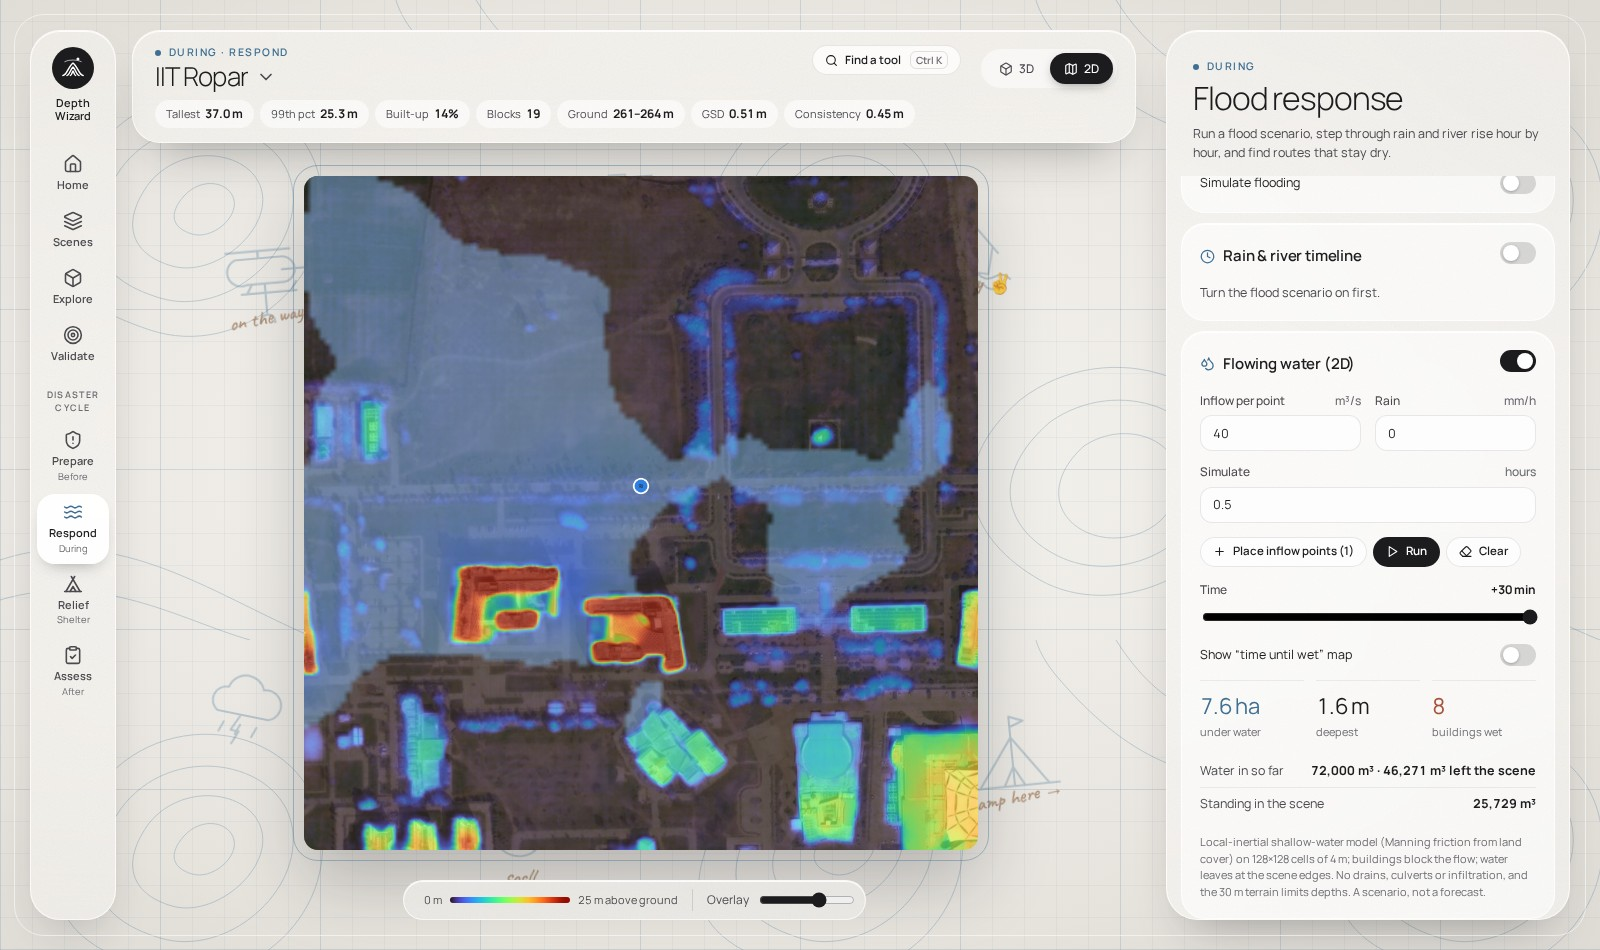
\includegraphics[width=\linewidth]{s_flow.jpg}\caption{Flowing water from an inflow point}\end{subfigure}\hfill
\begin{subfigure}{0.485\linewidth}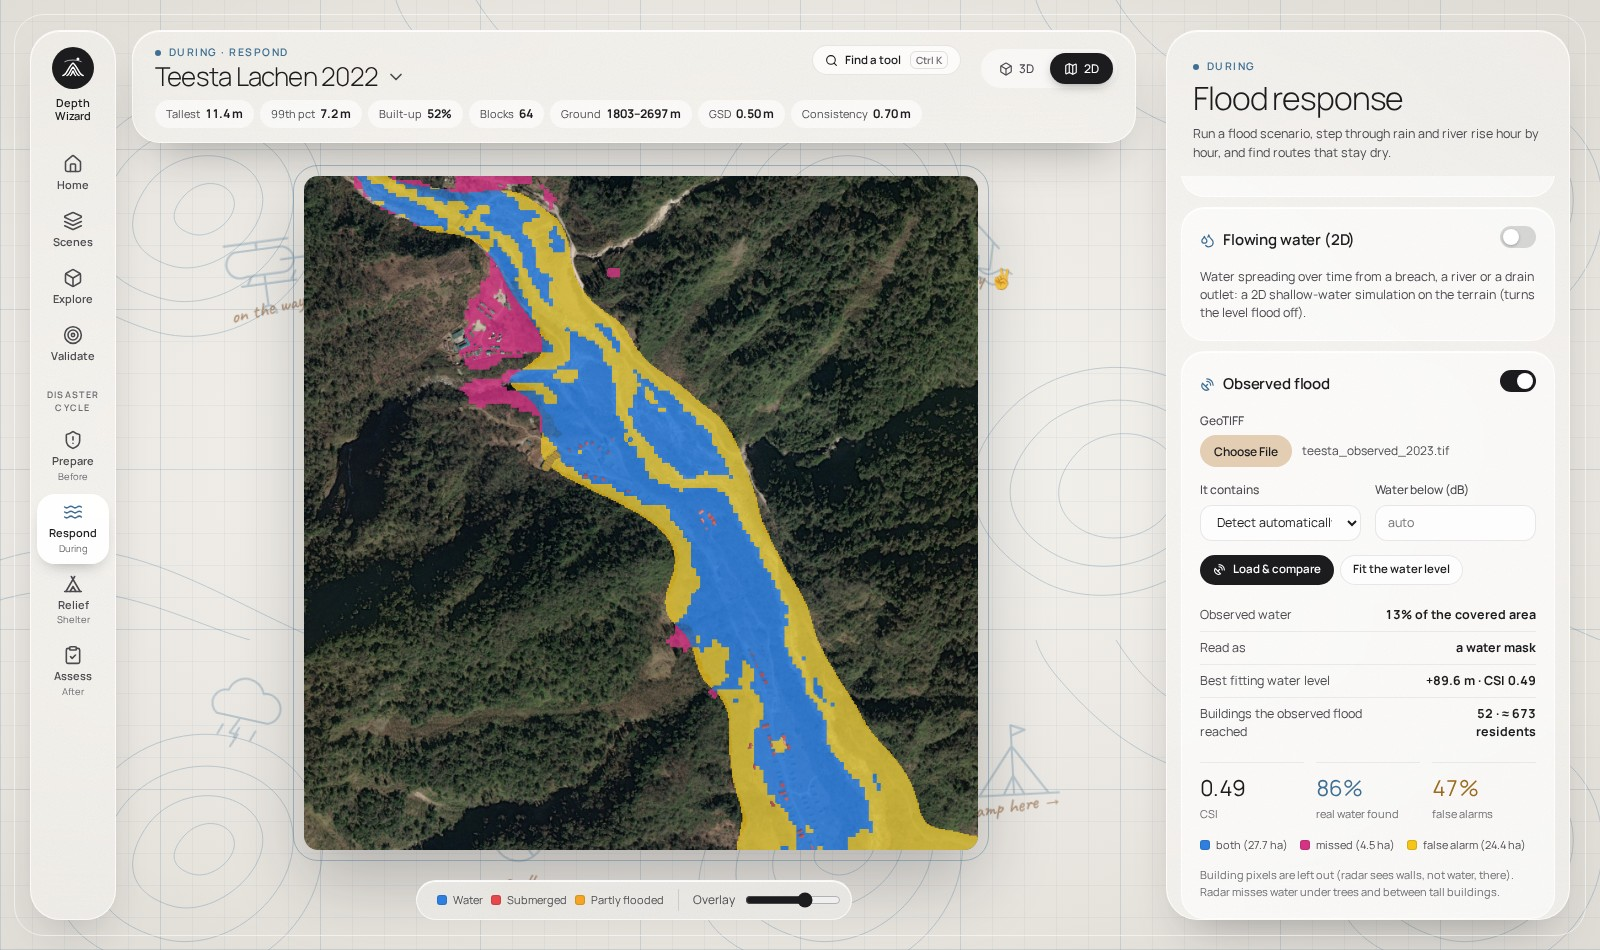
\includegraphics[width=\linewidth]{s_obs.jpg}\caption{Observed flood vs scenario, Teesta 2023}\end{subfigure}\\[6pt]
\begin{subfigure}{0.485\linewidth}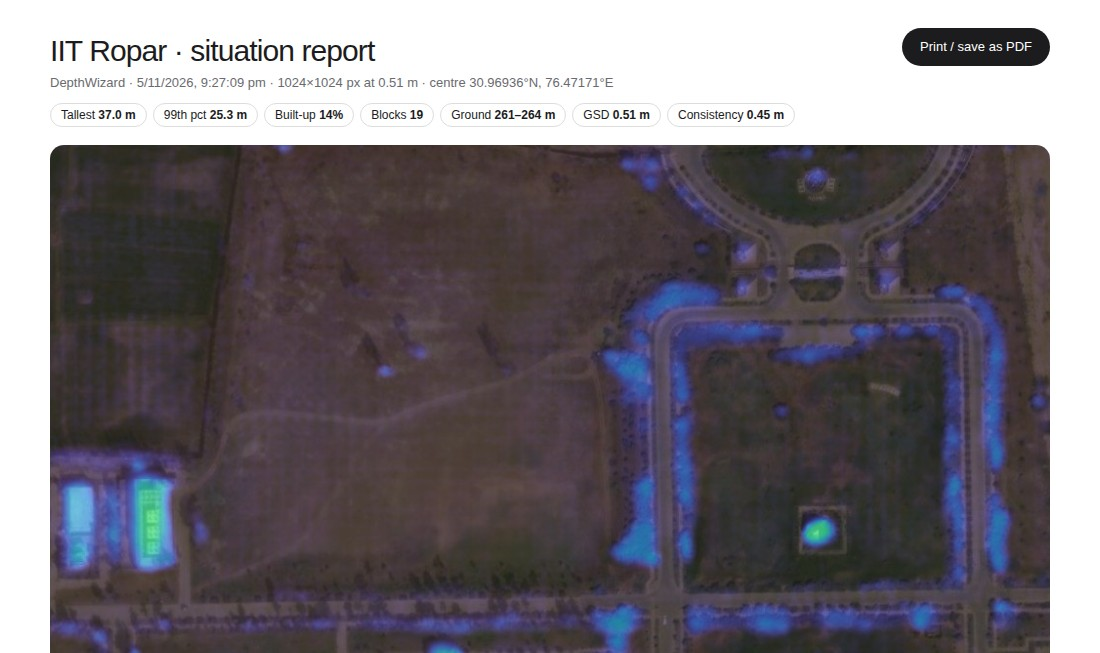
\includegraphics[width=\linewidth]{s_report.jpg}\caption{Situation report}\end{subfigure}\hfill
\begin{subfigure}{0.485\linewidth}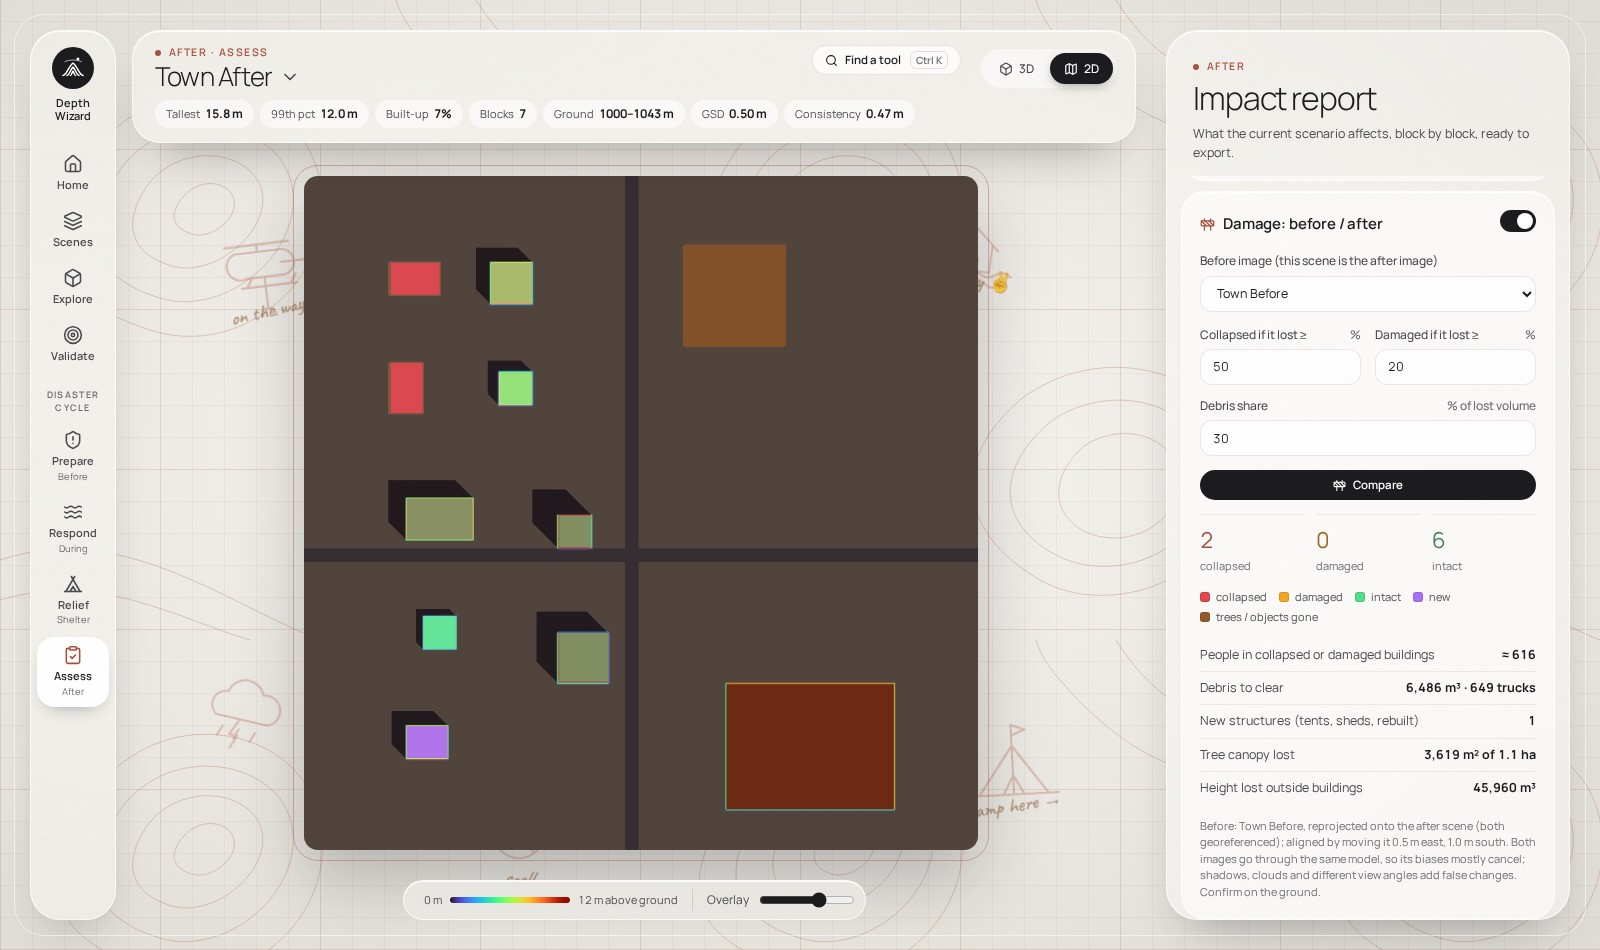
\includegraphics[width=\linewidth]{s_damage.jpg}\caption{Damage before/after (built-in test scene)}\end{subfigure}
\caption{Tools running in the application. Panels (a)--(e) and (g): the IIT Ropar campus; (f): the Teesta valley with the 2023 damage map (Section~\ref{sec:teesta}); (h): a built-in test scene with known collapsed buildings, because no real before/after pair has been processed yet.}
\label{fig:tools}
\end{figure}

% =====================================================================
\psection{Test Data and Protocol}{how we measured}
\label{sec:data}

All tests are zero-shot: the model never saw these places in training and nothing was tuned on them. Table~\ref{tab:data} lists the test data.

\begin{table}[!htbp]
\centering\small
\caption{Test data.}
\label{tab:data}
\begin{tabularx}{\linewidth}{@{}p{2.4cm}p{3.6cm}p{2.9cm}Y@{}}
\toprule
Name & Images & Truth from & Size and use \\
\midrule
GAMUS~\cite{xiong2023gamus} & Aerial photos, 0.33\m & Aircraft lidar & 150 tiles in three US cities; accuracy and error ranges \\
Geopose~\cite{christie2021geopose} & Satellite images & Lidar & 300 tiles each, Atlanta and Buenos Aires; published results \\
India & Satellite, 0.31--0.5\m & ICESat-2 and GEDI & 8 sites: two each of town, sparse land, hills and forest \\
Porto Alegre & Maxar, before the 2024 flood~\cite{maxar} & Mapped flood extent & 4 windows of $320\times320$\m; flood test \\
Teesta & Maxar 2022; Sentinel-2~\cite{drusch2012sentinel2} & Before/after change & 12\,km of valley; case study \\
\bottomrule
\end{tabularx}
\end{table}

With our height $\hat h_i$ and the true height $h_i$ at $N$ points we report
\begin{equation}
\mathrm{MAE} = \frac{1}{N}\sum_{i=1}^{N}\bigl|\hat h_i - h_i\bigr|,\qquad
\mathrm{bias} = \frac{1}{N}\sum_{i=1}^{N}\bigl(\hat h_i - h_i\bigr),\qquad
\mathrm{RMSE} = \sqrt{\frac{1}{N}\sum_{i=1}^{N}\bigl(\hat h_i - h_i\bigr)^2}.
\label{eq:metrics}
\end{equation}
MAE is the average size of the error, bias says whether we are too high or too low on average, and RMSE weighs large errors more. Every value is a mean over tiles or sites with a 95\% confidence range from 2,000 bootstrap resamples, shown in brackets, and is compared with a baseline measured at the same points. At the Indian sites, laser tracks alternate between correcting the map and checking it, so no laser point is used for both. Every number in this paper is recorded, with the file that produced it, in the project's claims register.

% =====================================================================
\psection{Results}{how accurate, and where}
\label{sec:results}

Unless stated otherwise, results in this section are for the published RS3DAda model inside DepthWizard.

\subsection{Height accuracy}

\begin{table}[!htbp]
\centering\small
\caption{Average height error in metres (lower is better), against a simple baseline at the same points; 95\% confidence ranges in brackets.}
\label{tab:accuracy}
\begin{tabularx}{\linewidth}{@{}Ycccc@{}}
\toprule
Test & Size & DepthWizard & Baseline \\
\midrule
\multicolumn{4}{@{}l}{\textit{Aerial photos, against aircraft lidar}} \\
Every point & 150 tiles & 3.90 [3.24, 4.66] & 5.65 (flat) \\
Buildings & 1,450 & 3.57 [3.08, 4.06] & 10.54 (flat) \\
Town / forest / open land & 137--148 tiles & 2.90 / 6.67 / 0.96 & 5.66 / 8.70 / 0.55 \\
\addlinespace
\multicolumn{4}{@{}l}{\textit{Satellite images}} \\
Atlanta & 300 tiles & 5.99 [5.57, 6.43] & 5.67 (published) \\
Buenos Aires & 300 tiles & 1.94 [1.86, 2.03] & 2.01 (published) \\
\addlinespace
\multicolumn{4}{@{}l}{\textit{India, against NASA lasers}} \\
Object heights, ICESat-2 & 8 sites & 4.85 [3.04, 6.69] & 8.25 (height 0) \\
Tree and roof heights, GEDI & 7 sites & 9.93 [4.86, 15.42] & 16.89 (height 0) \\
\bottomrule
\end{tabularx}
\end{table}

For buildings, DepthWizard's heights are about three times closer to the truth than the flat-ground guess (Table~\ref{tab:accuracy}); at Indian sites they are almost twice as close as guessing zero; and on satellite images they agree with the original authors' published results within our confidence ranges, so our software does not lose accuracy. Figure~\ref{fig:mae} breaks the error down by type of surface: the gain comes from buildings and trees, while on roads and bare ground, where the true height is close to zero, the flat guess is already right and slightly better. Figures~\ref{fig:gamus} and~\ref{fig:delhi} show what the heights look like.

\begin{figure}[!htbp]
\centering
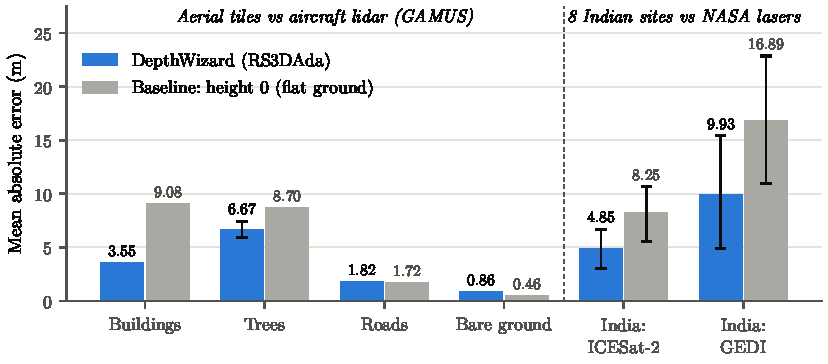
\includegraphics[width=\linewidth]{c_mae.pdf}
\caption{Average height error by type of surface. Left: aerial tiles against aircraft lidar. Right: Indian sites against NASA lasers, with 95\% confidence ranges.}
\label{fig:mae}
\end{figure}

\begin{figure}[!htbp]
\centering
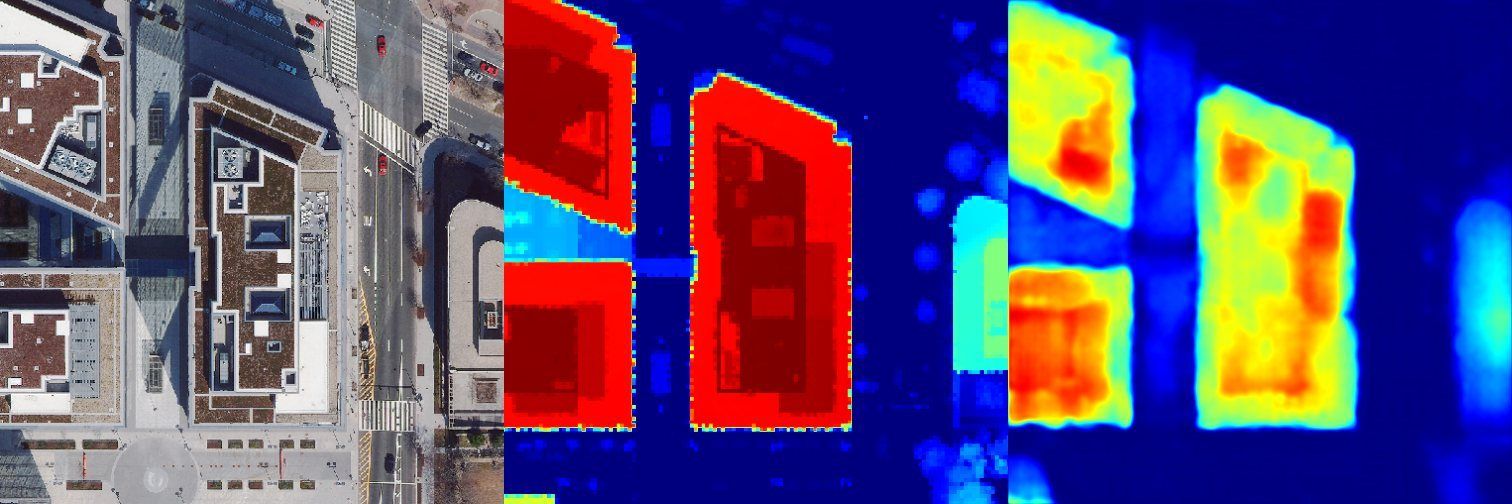
\includegraphics[width=\linewidth]{gamus.jpg}
\caption{One test tile: the aerial photo (left), the true heights from aircraft lidar (middle) and DepthWizard's heights from the photo alone (right). Red is tall, blue is low.}
\label{fig:gamus}
\end{figure}

\begin{figure}[!htbp]
\centering
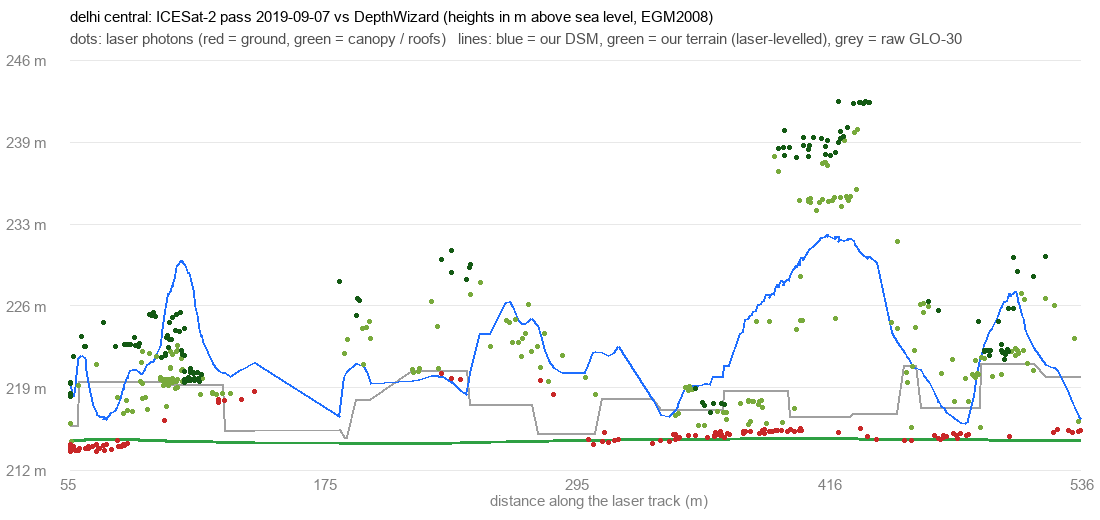
\includegraphics[width=0.8\linewidth]{delhi.png}
\caption{A slice through Delhi along a NASA laser track. Red dots: laser hits on the ground; green dots: hits on trees and roofs; blue line: our heights; green line: our ground level; grey line: the free GLO-30 map.}
\label{fig:delhi}
\end{figure}

\subsection{Comparison of height models}
\label{sec:compare}
We ran four models on the same 750 tiles (150 GAMUS, 300 Atlanta, 300 Buenos Aires), each cropped to the same centre and read four times with flips: RS3DAda, our Mamba student, and the relative and metric versions of Depth Anything~V2 (Large)~\cite{yang2024dav2}, a leading general-purpose depth model. Depth Anything gives relative depth, not heights in metres, so for a fair comparison every model is also scored after its output is fitted to the true heights with the best scale and offset for each tile (``aligned''); this shows how well a model finds \emph{where} things are tall, independent of units. Because every tile is cut to the same centre, the RS3DAda values differ slightly from Table~\ref{tab:accuracy}. Table~\ref{tab:compare} gives the results and Figure~\ref{fig:examples} shows typical tiles.

\begin{table}[!htbp]
\centering\small
\caption{Height models on the same 750 tiles: average error in metres (lower is better), cost on one GPU. ``As predicted'': heights used directly; ``aligned'': after the best scale and offset per tile.}
\label{tab:compare}
\begin{tabularx}{\linewidth}{@{}Ycccccc@{}}
\toprule
 & \multicolumn{3}{c}{As predicted} & \multicolumn{3}{c}{Aligned} \\
\cmidrule(lr){2-4}\cmidrule(l){5-7}
Model & GAMUS & Atlanta & B.\,Aires & GAMUS & Atlanta & B.\,Aires \\
\midrule
Flat ground (height 0) & 5.65 & 8.98 & 3.86 & -- & -- & -- \\
RS3DAda & \textbf{3.90} & \textbf{5.91} & \textbf{1.86} & \textbf{2.95} & \textbf{4.94} & \textbf{1.79} \\
DepthWizard-Mamba (ours) & 7.20 & 8.70 & 3.39 & 3.97 & 7.10 & 2.54 \\
Depth Anything V2, relative & -- & -- & -- & 3.25 & 5.64 & 2.18 \\
Depth Anything V2, metric & -- & -- & -- & 3.49 & 6.21 & 2.40 \\
\midrule
 & Parameters & Memory & \multicolumn{4}{l}{Speed} \\
\midrule
RS3DAda & 366.5\,M & 705\,MiB & \multicolumn{4}{l}{105 tiles per minute} \\
DepthWizard-Mamba (ours) & 40.7\,M & 78\,MiB & \multicolumn{4}{l}{546 tiles per minute} \\
Depth Anything V2, relative & 335.3\,M & 1{,}532\,MiB & \multicolumn{4}{l}{118 tiles per minute} \\
Depth Anything V2, metric & 335.3\,M & 650\,MiB & \multicolumn{4}{l}{134 tiles per minute} \\
\bottomrule
\end{tabularx}
\end{table}

RS3DAda is the most accurate model on every test, with or without alignment; the differences from Depth Anything~V2 are small but certain (relative version, aligned: $+0.30$, $+0.70$ and $+0.39\m$ worse on the three sets, all 95\% ranges above zero). The Mamba student is the cheapest model by far, but its first version is clearly less accurate: per tile it is 3.30\m{} [2.73, 3.92] worse than RS3DAda on GAMUS, 2.79\m{} on Atlanta and 1.53\m{} on Buenos Aires. It beats the flat-ground guess on the two satellite sets (by 0.28 and 0.47\m) but not on the aerial one, where it overestimates low ground by about 3\m. All models underestimate the tallest objects: above 20\m, RS3DAda is 19.1\m{} too low on GAMUS and the student 19.5\m.

\begin{figure}[!htbp]
\centering
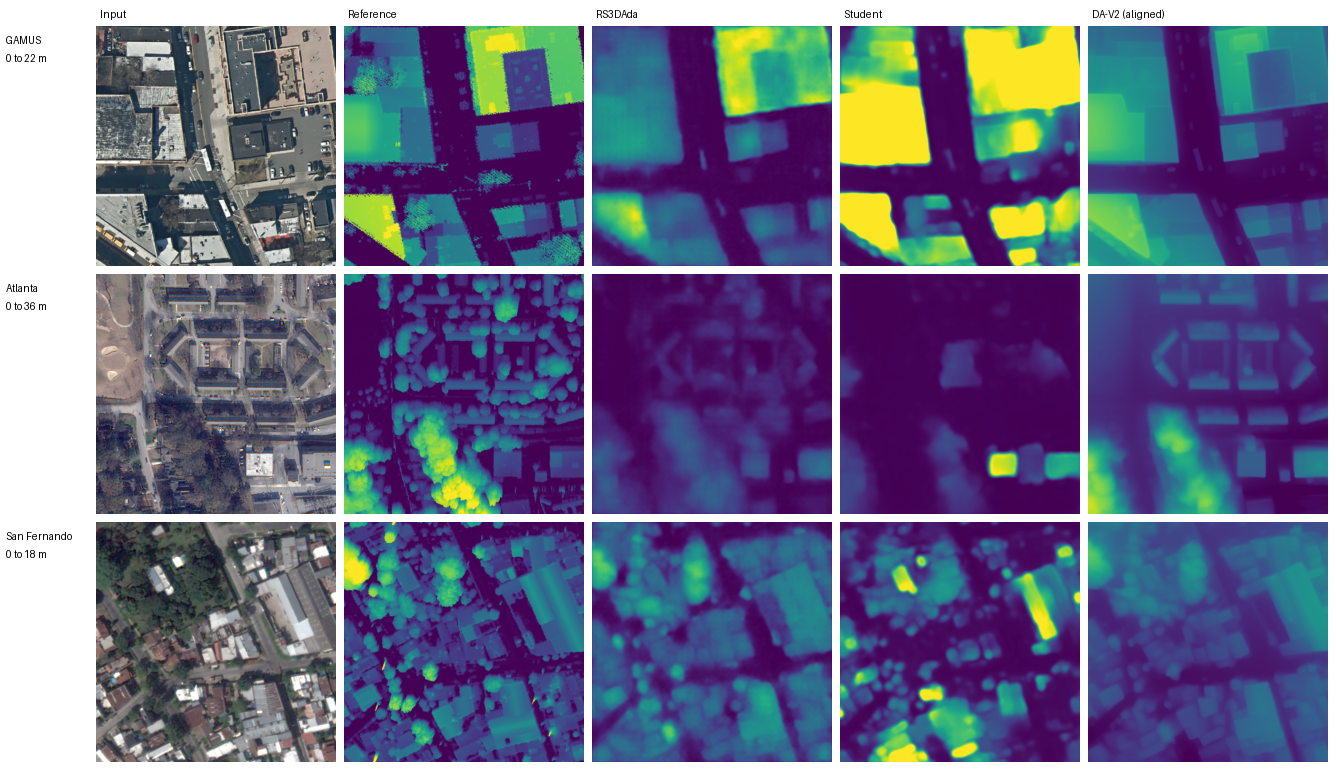
\includegraphics[width=\linewidth]{height_examples.png}
\caption{Typical tiles (the median tile for RS3DAda in each set): input, lidar reference, RS3DAda, our Mamba student and Depth Anything~V2 (relative, aligned). Rows: GAMUS, Atlanta, and San Fernando from the Buenos Aires set. Colour from 0 (dark) to the value on the left (yellow). The student finds buildings but overstates them on GAMUS and blurs small objects.}
\label{fig:examples}
\end{figure}

\subsection{Tall objects and error ranges}
Low objects are about right, but tall ones come out far too low (Figure~\ref{fig:height}a): above 20\m, heights are 16.26\m{} too low on aerial tiles, 16.80\m{} and 15.25\m{} too low in the two satellite cities, and 18.31\m{} too low in India. This is the main weakness of the published model. The 90\% error range of Eq.~\eqref{eq:conformal} held for 86.6\% (Washington DC), 83.3\% (New York) and 97.0\% (Philadelphia) of building blocks in cities it was not set on, with a half-width of about 6\m, and for 71\% of 96 Indian roofs. Figure~\ref{fig:height}b shows that it holds for low buildings but fails for tall ones, for the same reason; the app warns users about this.

\begin{figure}[!htbp]
\centering
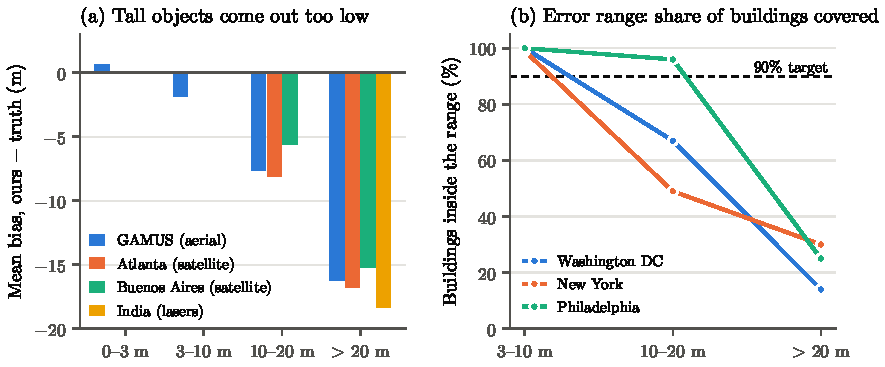
\includegraphics[width=\linewidth]{c_height.pdf}
\caption{(a) Average bias by true object height on aerial, satellite and Indian tests. (b) Share of building blocks whose true height falls inside the 90\% range, by height, in three cities not used to set the range.}
\label{fig:height}
\end{figure}

\subsection{Ground level and heights above sea level}
Removing rooftops and trees from the free terrain map halves the ground-level error in Indian towns, from 5.28\m{} to 2.36\m, slightly better than FABDEM's 2.80\m{} (Figure~\ref{fig:terrain}a). On sparse land all three maps agree; in the hills FABDEM is better; and under forest every map is about 20\m{} off, ours the most. Levelling to ICESat-2 removes the average offset of the ground map, from $+2.58\m$ to $-0.27\m$, but not its typical error (Table~\ref{tab:ground}). For floods, which depend on small height differences over a wide area, this offset is what matters: with laser levelling the flood map agreed far better with the real flood (Figure~\ref{fig:terrain}b, Section~\ref{sec:flood}).

\begin{figure}[!htbp]
\centering
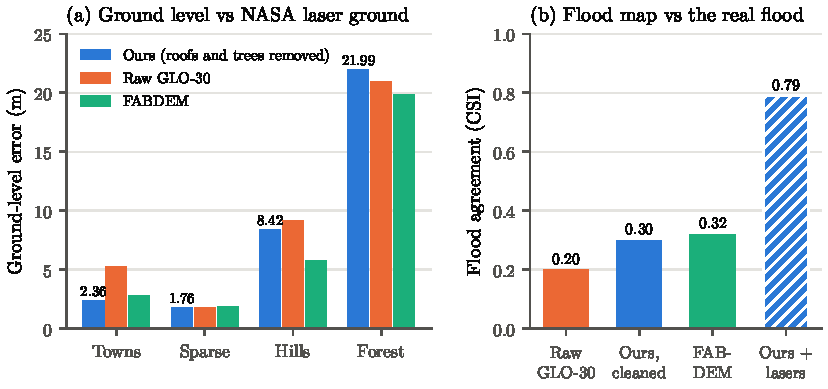
\includegraphics[width=\linewidth]{c_terrain.pdf}
\caption{(a) Ground-level error against NASA laser ground at the Indian sites, by landscape (two sites each). (b) Agreement between predicted and real flood maps in Porto Alegre with four ground maps; hatched: our map levelled to ICESat-2.}
\label{fig:terrain}
\end{figure}

\begin{table}[!htbp]
\centering\small
\caption{Ground level and heights above sea level at the Indian sites (error in m).}
\label{tab:ground}
\begin{tabularx}{\linewidth}{@{}Yccc@{}}
\toprule
Comparison & Sites & Ours & Alternative \\
\midrule
Ground vs held-out laser ground, current app & 5 & 3.73 [1.44, 6.69] & 3.86 (not levelled) \\
Average offset of the ground map & 5 & $-0.27$ & $+2.58$ (not levelled) \\
Ground vs all laser ground, not levelled & 8 & 8.63 & 9.31 GLO-30; 7.56 FABDEM \\
Surface vs all laser hits & 8 & 9.14 & 8.06 GLO-30 \\
Surface vs GEDI tree and roof tops & 7 & 5.97 & 8.39 GLO-30 \\
\bottomrule
\end{tabularx}
\end{table}

At individual laser spots our surface is not more accurate than the free 30\m{} surface map except on sparse land; what the photograph adds is detail at 0.5\m, which a 30\m{} map cannot have.

\subsection{Flood test: Porto Alegre, Brazil, May 2024}
\label{sec:flood}
We flooded the pre-flood heights of four areas and compared them with the mapped extent of the real flood on 6 May 2024. With the free terrain map the agreement was 0.20; with our cleaned map 0.30; with FABDEM 0.32; and with our map levelled to NASA lasers 0.79 (Figures~\ref{fig:terrain}b and~\ref{fig:poa}). Without levelling, over all seven areas, the agreement was 0.18, 0.47 and 0.48 for the free map, ours and FABDEM. This is a test of the method, not a forecast, and the areas are small.

\begin{figure}[!htbp]
\centering
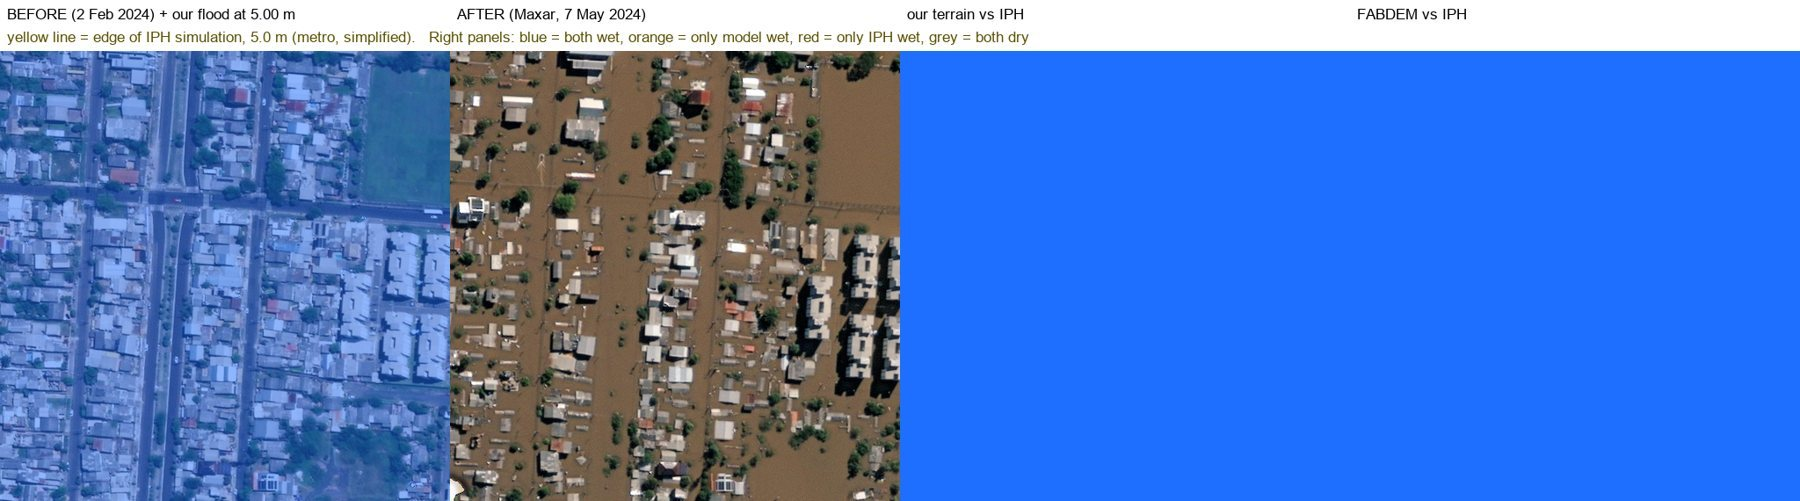
\includegraphics[width=\linewidth]{floodcmp.jpg}
\caption{Predicted versus real flood in Porto Alegre. Blue: both wet; orange: only our prediction wet; red: only the real flood wet. Imagery: Maxar Open Data (CC BY-NC 4.0).}
\label{fig:poa}
\end{figure}

\subsection{A real Indian disaster: the Teesta flood, Sikkim, 4 October 2023}
\label{sec:teesta}
On 4 October 2023 the South Lhonak glacial lake burst and sent a flood down the Teesta valley. Using only free public data, we compared Sentinel-2~\cite{drusch2012sentinel2} images from 20 November 2022 and 15 November 2023, the first cloud-free pair after the monsoon, with a pre-flood photograph of the Lachen valley~\cite{maxar}. Two standard indices separate vegetation and water:
\begin{equation}
\mathrm{NDVI} = \frac{\rho_{\mathrm{NIR}}-\rho_{\mathrm{red}}}{\rho_{\mathrm{NIR}}+\rho_{\mathrm{red}}},\qquad
\mathrm{MNDWI} = \frac{\rho_{\mathrm{green}}-\rho_{\mathrm{SWIR}}}{\rho_{\mathrm{green}}+\rho_{\mathrm{SWIR}}},
\label{eq:indices}
\end{equation}
where $\rho$ is the reflectance in each band. Ground counts as flood-damaged when it lies within 600\m{} of the river, has a slope under $25^\circ$, is cloud-free in both images, and either lost its vegetation (NDVI fell by more than 0.25 to below 0.3) or turned into water (MNDWI above zero only after the event). Figure~\ref{fig:teesta} and Table~\ref{tab:teesta} give the result.

\begin{figure}[!htbp]
\centering
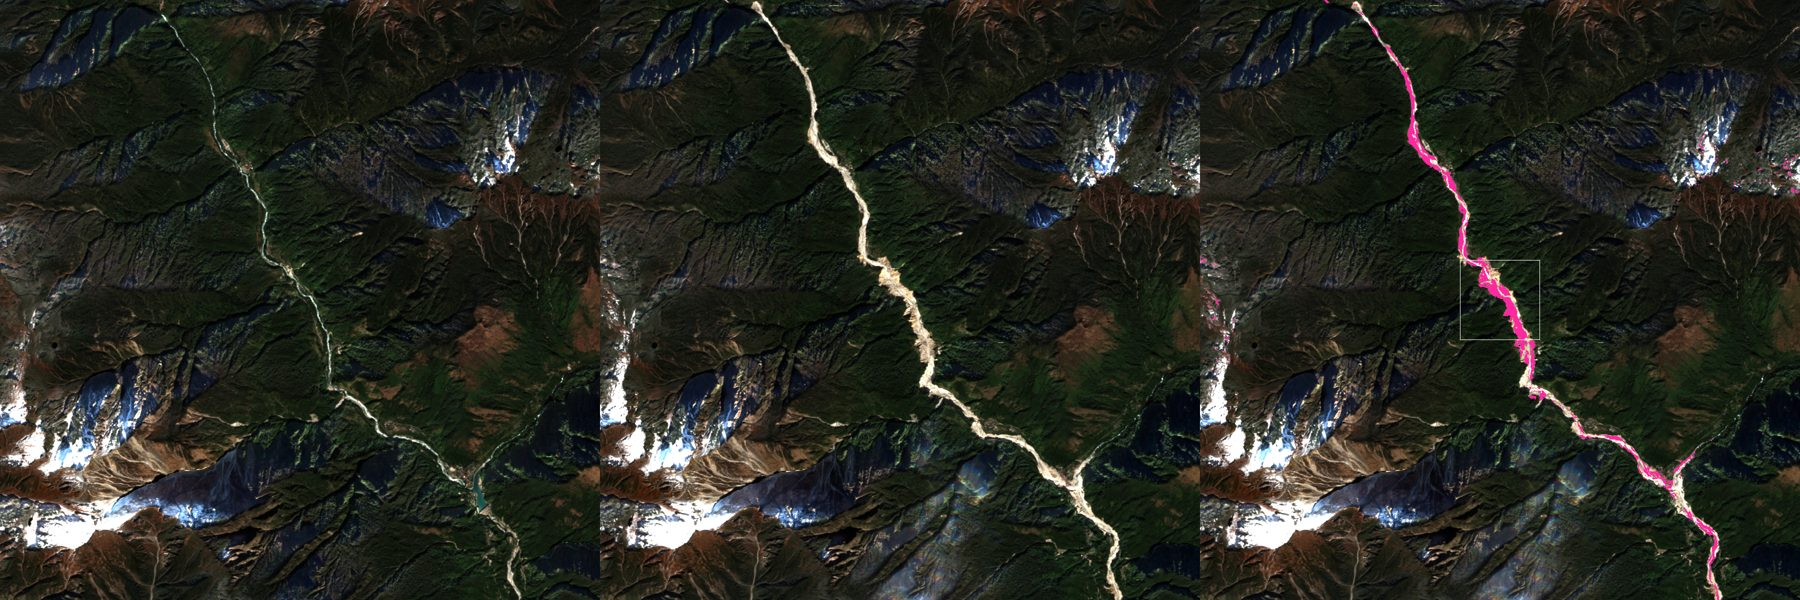
\includegraphics[width=\linewidth]{teesta.jpg}
\caption{The Teesta valley before (left) and after (middle) the flood; flood-damaged ground in magenta (right). White box: the area loaded into DepthWizard.}
\label{fig:teesta}
\end{figure}

\begin{table}[!htbp]
\centering\small
\caption{The Teesta flood, measured from Sentinel-2.}
\label{tab:teesta}
\begin{tabularx}{\linewidth}{@{}Yccc@{}}
\toprule
Measure & Before & After & Change \\
\midrule
Lake open water & 1.358\,km$^2$ & 1.28\,km$^2$ & $-5.7\%$ \\
Lake water murkiness (NIR reflectance) & 0.046 & 0.067 & $\times 1.5$ \\
Damaged ground, 12\,km of valley & -- & 1.281\,km$^2$ & of 52.85\,km$^2$ checked \\
Damaged ground, our area & -- & 0.328\,km$^2$ & 13\% of the area \\
\bottomrule
\end{tabularx}
\end{table}

The lake shrank only slightly but became much muddier: the outburst drained it downwards more than it changed its outline, so its area alone understates how much water escaped. We then ran DepthWizard on the pre-flood Lachen scene (3,200 $\times$ 3,200 pixels at 0.5\m, 559\m{} of relief, 64 buildings found) and loaded the damage map into the Observed-flood tool (Figure~\ref{fig:tools}f). The flood level that best matches the damage map gives a critical success index of 0.49: the scenario covers 86\% of the damaged ground, while 47\% of the ground it floods was not damaged. The damaged area reached 52 buildings, home to about 673 people by the app's floor-area estimate. A single water level is a crude model of a fast flood in a steep valley, which explains much of the over-flooding, and the damage map shows what the flood left behind a month later rather than its peak; its 10\m{} pixels suit areas, not single houses.

\subsection{What we tried, and what it changed}
Table~\ref{tab:ablation} records changes that were tested on the same data, including those that did not help and were therefore not kept.

\begin{table}[!htbp]
\centering\small
\caption{Tested changes and their effect.}
\label{tab:ablation}
\begin{tabularx}{\linewidth}{@{}p{4.3cm}Yl@{}}
\toprule
Change & Effect on the same test & Decision \\
\midrule
Four flipped readings, not one & Error $-0.064\m$ [$-0.101$, $-0.035$]; better on 114 of 150 tiles & Kept \\
Roof-point rule for lasers & Ground error 4.30\,$\to$\,2.63\m{} (Porto Alegre), 0.76\,$\to$\,0.59\m{} (Bengaluru); one area 2.15\,$\to$\,2.38\m & Kept \\
Refuse single-track levelling & Stopped a wrong 46.59\m{} shift in Silent Valley & Kept \\
Height recalibration curve & Better in two cities, worse in the third (1.86\,$\to$\,2.87\m) & Not kept \\
Resampling the input image & 3.08\m{} resampled vs 3.15\m{} native; not significant & Not kept \\
Denser levelling with GEDI & 4.18--4.24\m{} vs 4.02\m & Not kept \\
Error range per pixel & Held 81.4--96.1\% of the time; missed the target & Per building \\
\bottomrule
\end{tabularx}
\end{table}

\subsection{Software tests and speed}
Automated tests click through every tool on scenes whose true answers are known: 38 checks in the main interface and 36 in the older viewer, all passing. One full scene runs from upload to 3D in 42\,s on an 8\,GB Apple M3 laptop.

% =====================================================================
\psection{Discussion}{meaning, limits, next steps}
\label{sec:discussion}

\subsection{What the results mean}
From one photograph, DepthWizard gives building heights good to a few metres, a ground map that is far better than the free map in towns, and a flood picture that matches reality well once the ground is levelled with lasers. It is most reliable for low and medium buildings in towns, and least reliable for tall buildings and forests. Because every number carries a measured error and a baseline, a user can see in advance where to trust it.

\subsection{Limitations}

\begin{table}[!htbp]
\centering\small
\caption{Known limits and how DepthWizard deals with them today.}
\label{tab:limits}
\begin{tabularx}{\linewidth}{@{}YYY@{}}
\toprule
Limit & Effect & What we do \\
\midrule
Objects over 20\m{} are 15--18\m{} too low & Tall refuges look shorter & Warning on every result \\
Trees at 18--60\% of true height & Forest heights unreliable & Canopy map or GEDI correction \\
Ground under forest about 20\m{} off & Floods in forest unreliable & Flagged in the app \\
Mamba student less accurate so far & 7.20 vs 3.90\m{} on GAMUS & App keeps RS3DAda \\
Mamba model needs an NVIDIA card & Not in the laptop version & GPU servers only \\
Only two Indian sites per landscape & Wide confidence ranges & Ranges always reported \\
India's Cartosat images need a login & Not yet tested & Request to NRSC drafted \\
\bottomrule
\end{tabularx}
\end{table}

\subsection{Responsible use and licences}
All disaster outputs are scenarios meant to support planning, not forecasts, and are labelled so in the app. Population figures are estimated from building floor area, not from personal data. The RS3DAda weights were trained on non-commercial data, and FABDEM and the Maxar demonstration images are also non-commercial, so DepthWizard is suitable for research and government pilots; commercial use would need new weights or permissions.

\subsection{Next steps}
\begin{enumerate}
\item \textbf{Improve the Mamba model:} train longer, use the true-height term of Eq.~\eqref{eq:distill}, and adapt it to real images with RS3DAda's full recipe, until it matches RS3DAda's accuracy while keeping its five-fold speed.
\item \textbf{Improve trees and tall buildings:} measure the canopy and GEDI corrections on Indian forests, and use shadow lengths to correct tall buildings.
\item \textbf{Extend the Teesta study:} replace the single water level with the flowing-water model of Eq.~\eqref{eq:flow}, released from the lake, and score it against the damage map.
\item \textbf{Pilot} with one State Disaster Management Authority through a monsoon, validate on Cartosat imagery, and hand the code and results to NRSC and ISRO.
\end{enumerate}

% =====================================================================
\psection{Conclusion}{}

From one ordinary satellite photograph, combined with free terrain data and NASA's lasers, DepthWizard produces a 3D height map that disaster teams can use offline and check for themselves. Our main novelty is a Mamba-based height model that gives the same outputs as the published model while being nine times smaller and five times faster; its first version is not yet as accurate, so it is a promising start rather than a replacement. With the published model, DepthWizard beats simple guesses on every height test, halves the ground-level error in Indian towns, raises flood-map agreement from 0.30 to 0.79 with laser levelling, outperforms Depth Anything~V2 on the same tiles, and maps a real Indian disaster from public data. It does not yet replace a ground survey: very tall buildings come out too low and forests remain hard. Because every result comes with its error, users can see where to trust it.

% =====================================================================
\usection{Author Contributions}
\textbf{Himanshu Patel:} project set-up and processing pipeline; the Mamba-based model and distillation code; terrain cleaning, ICESat-2 levelling and the roof-point rule; evaluation protocol and claims register; user interface, landing page and the eighteen tools; Teesta case study; canopy-map and GEDI correction.
\textbf{Shlok Vaidya:} in-app height validation and control-point calibration; standalone installer; helipad finder and route search; training of the Mamba student; the comparison of RS3DAda, the Mamba student and Depth Anything~V2; application screenshots; benchmark reports and the October project report.

\subsection*{Acknowledgements}
We thank our mentors at IIT Ropar. Imagery: Maxar Open Data Program and ESA Copernicus Sentinel-2. Ground heights: Copernicus GLO-30. Laser data: NASA ICESat-2 and GEDI. Tree heights: Meta and the World Resources Institute.

\subsection*{Data and code availability}
The code, test scripts and claims register are in the project repository, \url{https://github.com/hima1323/terravista-depthwizard}. All test data are public and are cited in Table~\ref{tab:data}; each number in this paper is linked in the claims register to the file that produced it.

% =====================================================================
\begingroup
\small
\renewcommand{\refname}{References}
\titleformat{\section}[block]{\Large\bfseries}{}{0em}{}[{\vspace{-1.5pt}\titlerule[0.6pt]}]
\begin{thebibliography}{99}\setlength{\itemsep}{1pt}
\bibitem{gu2023mamba} A.~Gu and T.~Dao. Mamba: Linear-time sequence modeling with selective state spaces. \emph{arXiv:2312.00752}, 2023.
\bibitem{hatamizadeh2025mambavision} A.~Hatamizadeh and J.~Kautz. MambaVision: A hybrid Mamba-Transformer vision backbone. In \emph{Proc.\ CVPR}, 2025. arXiv:2407.08083.
\bibitem{song2024synrs3d} J.~Song, H.~Chen, W.~Xuan, J.~Xia and N.~Yokoya. SynRS3D: A synthetic dataset for global 3D semantic understanding from monocular remote sensing imagery. In \emph{NeurIPS Datasets and Benchmarks}, 2024. arXiv:2406.18151.
\bibitem{oquab2023dinov2} M.~Oquab \emph{et al.} DINOv2: Learning robust visual features without supervision. \emph{arXiv:2304.07193}, 2023.
\bibitem{hinton2015distilling} G.~Hinton, O.~Vinyals and J.~Dean. Distilling the knowledge in a neural network. \emph{arXiv:1503.02531}, 2015.
\bibitem{ranftl2021dpt} R.~Ranftl, A.~Bochkovskiy and V.~Koltun. Vision transformers for dense prediction. In \emph{Proc.\ ICCV}, 2021.
\bibitem{esa2021glo30} European Space Agency. \emph{Copernicus DEM GLO-30}, 2021. \copyright~DLR e.V. 2010--2014 and \copyright~Airbus Defence and Space GmbH 2014--2018.
\bibitem{hawker2022fabdem} L.~Hawker \emph{et al.} A 30\,m global map of elevation with forests and buildings removed. \emph{Environmental Research Letters}, 17, 2022.
\bibitem{neumann2019icesat2} T.~A. Neumann \emph{et al.} The Ice, Cloud, and Land Elevation Satellite-2 mission: A global geolocated photon product derived from the ATLAS instrument. \emph{Remote Sensing of Environment}, 233, 2019.
\bibitem{neuenschwander2019atl08} A.~Neuenschwander and K.~Pitts. The ATL08 land and vegetation product for the ICESat-2 mission. \emph{Remote Sensing of Environment}, 221, 2019.
\bibitem{dubayah2020gedi} R.~Dubayah \emph{et al.} The Global Ecosystem Dynamics Investigation: High-resolution laser ranging of the Earth's forests and topography. \emph{Science of Remote Sensing}, 1, 2020.
\bibitem{tolan2024canopy} J.~Tolan \emph{et al.} Very high resolution canopy height maps from RGB imagery using self-supervised vision transformer and convolutional decoder trained on aerial lidar. \emph{Remote Sensing of Environment}, 300, 2024.
\bibitem{bates2010inertial} P.~D. Bates, M.~S. Horritt and T.~J. Fewtrell. A simple inertial formulation of the shallow water equations for efficient two-dimensional flood inundation modelling. \emph{Journal of Hydrology}, 387, 2010.
\bibitem{otsu1979} N.~Otsu. A threshold selection method from gray-level histograms. \emph{IEEE Transactions on Systems, Man, and Cybernetics}, 9(1), 1979.
\bibitem{bis14496} Bureau of Indian Standards. \emph{IS 14496 (Part 2): 1998, Preparation of landslide hazard zonation maps in mountainous terrains: Guidelines}.
\bibitem{lei2018conformal} J.~Lei, M.~G'Sell, A.~Rinaldo, R.~J. Tibshirani and L.~Wasserman. Distribution-free predictive inference for regression. \emph{Journal of the American Statistical Association}, 113, 2018.
\bibitem{dijkstra1959} E.~W. Dijkstra. A note on two problems in connexion with graphs. \emph{Numerische Mathematik}, 1, 1959.
\bibitem{threejs} three.js authors. three.js: JavaScript 3D library. \url{https://threejs.org}.
\bibitem{xiong2023gamus} Z.~Xiong \emph{et al.} GAMUS: A geometry-aware multi-modal semantic segmentation benchmark for remote sensing data. \emph{arXiv:2305.14914}, 2023.
\bibitem{christie2021geopose} G.~Christie \emph{et al.} Single view geocentric pose in the wild. In \emph{CVPR Workshops (EarthVision)}, 2021.
\bibitem{maxar} Maxar Technologies. Open Data Program: India Floods October 2023; Brazil Floods 2024. CC BY-NC 4.0.
\bibitem{yang2024dav2} L.~Yang, B.~Kang, Z.~Huang, Z.~Zhao, X.~Xu, J.~Feng and H.~Zhao. Depth Anything V2. In \emph{NeurIPS}, 2024. arXiv:2406.09414.
\bibitem{song2025sparse} J.~Song, H.~Chen and N.~Yokoya. Enhancing monocular height estimation via sparse LiDAR-guided correction. \emph{arXiv:2505.06905}, 2025.
\bibitem{drusch2012sentinel2} M.~Drusch \emph{et al.} Sentinel-2: ESA's optical high-resolution mission for GMES operational services. \emph{Remote Sensing of Environment}, 120, 2012.
\end{thebibliography}
\endgroup

% =====================================================================
\appendix
\renewcommand{\thetable}{A\arabic{table}}\setcounter{table}{0}
\renewcommand{\thefigure}{A\arabic{figure}}\setcounter{figure}{0}
\psection{Detailed Results}{}

\begin{table}[!htbp]
\centering\small
\caption{Further results on the 150 aerial lidar tiles (GAMUS).}
\begin{tabularx}{\linewidth}{@{}p{6cm}Y@{}}
\toprule
Measure & Value [95\% confidence range] \\
\midrule
RMSE & 5.58\m{} [4.82, 6.40] \\
Bias & $-2.61\m$ [$-3.41$, $-1.87$] \\
Correlation with lidar & 0.61 [0.57, 0.65] \\
Error by city & DC 5.16 [3.77, 6.75]; New York 4.69 [3.49, 5.99]; Philadelphia 1.86 [1.44, 2.39] \\
Objects taller than 3\m & 6.65\m{} [5.90, 7.44]; baseline 11.10\m \\
Points within $\pm2$\m & 61\%; baseline 54\% \\
Trees, predicted / true height & DC 0.20; New York 0.18; Philadelphia 0.60 \\
Disagreement of the four readings vs error & Rank correlation 0.44 overall; $-0.03$ above 3\m \\
\bottomrule
\end{tabularx}
\end{table}

\begin{table}[!htbp]
\centering\small
\caption{Indian sites by landscape: mean of two sites each, error in m.}
\begin{tabularx}{\linewidth}{@{}Yccc@{}}
\toprule
Landscape & Ground: ours / GLO-30 / FABDEM & Surface: ours / GLO-30 & Height: error, bias \\
\midrule
Town & 2.36 / 5.28 / 2.80 & 5.47 / 4.98 & 4.49, $-1.19$ \\
Sparse & 1.76 / 1.80 / 1.82 & 2.10 / 2.29 & 1.56, $+0.84$ \\
Hills & 8.42 / 9.20 / 5.74 & 8.57 / 7.75 & 8.25, $-5.12$ \\
Forest & 21.99 / 20.97 / 19.87 & 20.40 / 17.21 & 5.10, $-3.50$ \\
\bottomrule
\end{tabularx}
\end{table}

\begin{figure}[!htbp]
\centering
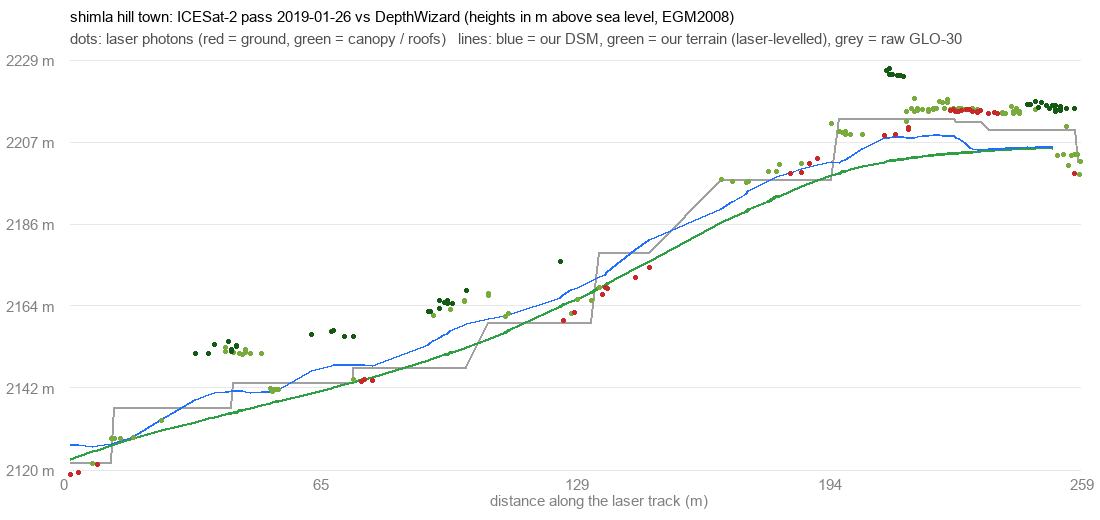
\includegraphics[width=0.8\linewidth]{shimla.png}
\caption{A slice through Shimla along a NASA laser track. Red dots: laser hits on the ground; green dots: hits on trees and roofs; blue line: our heights; green line: our ground level; grey line: the free GLO-30 map.}
\end{figure}

\end{document}
